\documentclass[a4paper,11pt]{ltjsarticle}
\usepackage{nomal_preamble}
\usepackage{anyfontsize}
\usepackage{multirow}
\usepackage{wrapfig}
\usepackage{tikz-3dplot}
\usetikzlibrary{angles,quotes}

\newcommand{\dlim}[2]{\displaystyle{\lim_{#1 \to #2}\:}}
\newcommand{\dint}[2]{\displaystyle{\int_{#1}^{#2}}}
\def\tick#1#2{\draw[thick] (#1)++(#2:0.12) --++ (#2-180:0.24)}
\def\N{100} % number of samples

\title{物理学概論Ⅰ\ 解説}
\author{ほうじ茶}
\date{}

\begin{document}

\pagestyle{fancy}
\lhead{\ 目次と付録}
\rhead{}
\cfoot{\thepage}

\maketitle
\tableofcontents

\vs{12}

\begin{center}
  目次をクリックすると，対応したページに遷移します．
\end{center}

\subsection*{留意事項}

\begin{enumerate}
  \item 本資料は講義資料や板書を基に作成をしており，実際に使われない言葉や記号が出てきます．
  \item 講義の順番にはなっていません．理解しやすいと思う順に記述しています．
  \item 自身の好み（独断と偏見）で作成しているので，旧字体やベクトルを行列で記載している箇所があります．
  \item 最重要事項または強調したい箇所には，\colorbox{yellow}{　　}\ で示しています．
  \item 色付き文字は重要事項または分かりやすくしたい箇所です．
  \item 第13・14回の問題演習は，提出なしのため作成はしていません．
  \item 定期試験は過去問からほぼ同等の問題が出るため，過去問を完璧にすることを推奨します．
  \item 物理学概論Ⅱの定期試験\ 大問5に力学（水平投射）問題が出るので，水平投射の解法は忘れないように．
\end{enumerate}

\subsection*{ベクトルかスカラーか}

物理学の世界では，ベクトル量なのかスカラー量なのかシビアに見られるのでここに簡単に記しておく．
ベクトルは高校までは上に矢印\ $\vec{r}$で表していたが，一般的には太字\ $\bm{r}$で記述する．

座標\ $(a \quad b \quad c)$のように記述されているものは，vectorである．
scalarを束にしたものがvector，vectorを束にしたものがmatrixである．
そのため，座標表記されたそれぞれ$a$，$b$，$c$はscalarだといえる．
また，$t$についての函数として表したいので$r(t)$の形もしばしば用いられる．
この記号の場合は確実に，vectorだ，scalarだといえるものを次に簡単にまとめておく．

\begin{table}[h]
  \centering
  \caption{vetcotかscalarか}
  \begin{tabular}{ccccccccccccc}
      \hline
      scalar & $m$ & $h$ & $x$ & $y$ & $z$ & $\dot{x}$ & $\dot{y}$ & $\dot{z}$ & $\ddot{x}$ & $\ddot{y}$ & $\ddot{z}$ & etc. \\
      vector & $\bm{r}$ & $\bm{v}$ & $\dot{\bm{r}}$ & $\bm{a}$ & $\ddot{\bm{r}}$ & etc.  & & & & & & \\
      \hline
  \end{tabular}
\end{table}

\clearpage

\pagestyle{fancy}
\lhead{\ 初等数学}
\rhead{}
\cfoot{\thepage}

\section{初等数学}

物理学においての最低限の数学を扱う．

\subsection{ベクトル}

簡単なイメージとしては，$x$軸，$y$軸のある座標のようなもの．
2次元の大きさ，すなわち「2つ以上の大きさの組」により\textbf{向き}が定まる．
考えるときには，$x$軸方向，$y$軸方向，（あれば$z$軸方向）を分離して考えることが大切である．
一般に\textbf{ベクトル量}と呼ばれる．また，今まで扱ってきたものは，「大きさ」しか持たない\textbf{スカラー量}というものである．

\subsubsection{ベクトルの加減法}

言葉で説明するなら，矢印の終点ともう一方の矢印の始点を合わせ，一つの折れ線矢印と見なし始点と終点を線で結ぶ．減法の場合は，矢印を逆（逆ベクトル）にしてから足す．
ほかに始点同士を揃えて平行四辺形にする方法もあり，運動方程式を解く際の分力を求めるのに最適である．

\hs{0}

\begin{center}
\begin{tikzpicture}
  \draw [-Stealth,thick] (0,0)--(1,2);
  \node [above left] at ($(0,0)!0.5!(1,2)$) {$\bm{b}$};
  \draw [-Stealth,thick] (1,0)--(4,0);
  \node [below] at ($(1,0)!0.5!(4,0)$) {$\bm{a}$};
  \draw [-Stealth,thick] (8,0)--(9,2);
  \node [right] at ($(8,0)!0.5!(9,2)$) {$\bm{b}$};
  \draw [-Stealth,thick] (5,0)--(8,0);
  \node [below] at ($(5,0)!0.5!(8,0)$) {$\bm{a}$};
  \draw [-Stealth,very thick,cyan] (5,0)--(9,2);
  \node [above left,cyan] at ($(5,0)!0.5!(9,2)$) {$\bm{a}+\bm{b}$};
  \draw [-Stealth,thick] (10,0)--(11,2);
  \node [above left] at ($(10,0)!0.5!(11,2)$) {$\bm{b}$};
  \draw [-Stealth,thick] (10,0)--(13,0);
  \node [below] at ($(10,0)!0.5!(13,0)$) {$\bm{a}$};
  \draw [dashed] (11,2)--(14,2)--(13,0);
  \draw [-Stealth,very thick,cyan] (10,0)--(14,2);
  \node [below right,cyan] at ($(10,0)!0.5!(14,2)$) {$\bm{a}+\bm{b}$};
\end{tikzpicture}
\end{center}

\vspace{-10pt}

\subsubsection{単位ベクトル}

ユークリッド空間（実数を$n$個並べた全体の集合）において，3つの直交座標をそれぞれ$x$軸，$y$軸，$z$軸とする．
そのなかで大きさを「1」に仕立てたベクトルを単位ベクトルという．
（単位○○は基本的に，○○の大きさを「1」に仕立てたもののことである．）

また，$x$軸と平行な単位ベクトルを$\bm{i}$，$y$軸と平行な単位ベクトルを$\bm{j}$，$z$軸と平行な単位ベクトルを$\bm{k}$とする．

\subsubsection{ベクトルの成分表示}

単位ベクトルと係数倍を用いて，一般にベクトルを次のような式で表せる．

\begin{equation}
  \bm{a}=A \bm{i}+B \bm{j}+C \bm{k}
\end{equation}

また，係数を座標のように表して，

\begin{equation}
  \bm{a}=(A \quad B \quad C)
\end{equation}

とも表せる．

\clearpage

\subsection{第1回\ 問題演習}

\begin{center}
\begin{tikzpicture}[scale=0.8]
  \draw[step=1,gray,very thin] (-3,-1) grid (6,6);
  \draw[-latex,thick] (-3,0) --(6,0);
  \draw[-latex,thick] (0,-1) --(0,6);
  \node[below] at (6,0) {$x$};
  \node[left] at (0,6) {$y$}; 
  \draw[-Stealth,very thick] (-1,2)--(-2,4);
  \node[above right] at ($(-1,2)!0.5!(-2,4)$) {$\bm{b}$};
  \draw[-Stealth,very thick] (1,5)--(1,1);
  \node[right] at ($(1,5)!0.5!(1,1)$) {$\bm{c}$};
  \draw[-Stealth,very thick] (2,1)--(5,3);
  \node[below right] at ($(2,1)!0.5!(5,3)$) {$\bm{a}$};
\end{tikzpicture}
\end{center}

\begin{enumerate}
  \item ベクトル$\bm{i}$，$\bm{j}$，$\bm{a}+\bm{b}$を図示しなさい．

  \begin{center}
    \begin{tikzpicture}[scale=0.8]
      \draw[step=1,gray,very thin] (-1,0) grid (6,6); 
      \draw[-Stealth,very thick] (5,3)--(4,5);
      \node[above right] at ($(5,3)!0.5!(4,5)$) {$\bm{b}$};
      \draw[-Stealth,very thick] (2,1)--(5,3);
      \node[below right] at ($(2,1)!0.5!(5,3)$) {$\bm{a}$};
      \draw[-Stealth,very thick,cyan] (0,5)--(1,5);
      \draw[-Stealth,very thick,cyan] (2,1)--(4,5);
      \node[above left,cyan] at ($(2,1)!0.5!(4,5)$) {$\bm{a}+\bm{b}$};
      \node[below,cyan] at ($(0,5)!0.5!(1,5)$) {$\bm{i}$};
      \draw[-Stealth,very thick,cyan] (0,2)--(0,3);
      \node[left,cyan] at ($(0,2)!0.5!(0,3)$) {$\bm{j}$};
    \end{tikzpicture}
  \end{center}

  \item ベクトル$\bm{a}$，$\bm{b}$，$\bm{c}$，$\bm{a}+\bm{b}$，$\bm{i}$，$\bm{j}$の成分表示を答えなさい．

  \begin{equation}
    \renewcommand{\arraystretch}{2}
    \begin{array}{rclrcl}
      \bm{a}
      &=&
      (3 \quad 2)
      &
      \bm{a}+\bm{b}
      &=&
      (2 \quad 4)
      \\
      \bm{b}
      &=&
      (-1 \quad 2)
      &
      \bm{i}
      &=&
      (1 \quad 0)
      \\
      \bm{c}
      &=&
      (0 \quad -4)
      &
      \bm{j}
      &=&
      (0 \quad 1)
    \end{array}
  \end{equation}

\clearpage

  \item スカラー積（内積）$\bm{a \cdot a}$と$\bm{a \cdot b}$を答えなさい．

  \begin{equation}
    \renewcommand{\arraystretch}{2}
    \begin{array}{rcl}
      \bm{a \cdot a}  &=& 3 \cdot 3 + 2 \cdot 2 \\
                      &=& 9+4 \\
                      &=& 13 \\
      \bm{a \cdot b}  &=& 3 \cdot (-1) + 2 \cdot 2 \\
                      &=& -3+4 \\
                      &=& 1
    \end{array}
  \end{equation}

  \item ベクトル$\bm{a}$の大きさを答えなさい．
  
  \begin{equation}
    \renewcommand{\arraystretch}{2}
    \begin{array}{rcl}
      |\bm{a}|  &=& \sqrt{\bm{a \cdot a}} \\
                &=& \sqrt{3 \cdot 3 + 2 \cdot 2} \\
                &=& \sqrt{9+4} \\
                &=& \sqrt{13}
    \end{array}
  \end{equation}

  \item ベクトル$\bm{v}_0$の大きさは$28$である．$\bm{v}_0$を成分表示せよ．
  
  \begin{center}
    \begin{tikzpicture}[scale=1.5, rotate=0]
      \coordinate (A) at (2,1.5) {};
      \coordinate (B) at (0,0) {};
      \coordinate (C) at (3,0) {};
      \coordinate (D) at (1,0) {};
      \coordinate (E) at (0,2) {};
      \draw [-Stealth,very thick,cyan] (B)--(A) node [above right] at (A) {$\bm{v}_0$};
      \draw [-latex,thick] (B)--(C) node [below] at (C) {$x$};
      \draw [-latex,thick] (B)--(E) node [left] at (E) {$y$};
      \pic["$30^{\circ}$",draw,angle radius=8mm,angle eccentricity=1.6] {angle = C--B--A};
  \end{tikzpicture}
  \end{center}

$\bm{v}_0$の成分表示は三角函数を用いて，

  \begin{equation}
    \renewcommand{\arraystretch}{2}
    \begin{array}{rcl}
      \bm{v}_0
      &=&
      (v_0 \cos{30^{\circ}} \quad v_0 \sin{30^{\circ}})
      \\
      &=&
      \left(28 \times \dfrac{\sqrt{3}}{2} \quad 28 \times \dfrac{1}{2}\right)
      \\
      &=&
      (14 \sqrt{3} \quad 14)
    \end{array}
  \end{equation}  

\clearpage

  \item ベクトル$\bm{G}$の大きさは$G$である．$\bm{G}$を成分表示せよ．

    \begin{figure}[htbp]
      \centering
      \begin{tabular}{ccc}
        \begin{minipage}[t]{0.3\linewidth}
          \begin{tikzpicture}[scale=1.3, rotate=233]
            \coordinate (A) at (2,1.5) {};
            \coordinate (B) at (0,0) {};
            \coordinate (C) at (3,0) {};
            \coordinate (D) at (1,0) {};
            \coordinate (E) at (0,2) {};
            \draw [-Stealth,very thick,cyan] (B)--(A) node [below] at (A) {$\bm{G}$};
            \draw [-latex,thick] (B)--(C) node [below] at (C) {$x$};
            \draw [-latex,thick] (E)--(B) node [left] at (B) {$y$};
            \pic["$\theta$",draw,angle radius=5mm,angle eccentricity=1.5] {angle = A--B--E};
        \end{tikzpicture}
        \end{minipage}
        &
        \hspace{20pt} \raisebox{0.12\textwidth}{$\Longrightarrow$} \hspace{20pt}
        &
        \begin{minipage}[t]{0.3\linewidth}
          \begin{tikzpicture}[scale=1.5, rotate=0]
            \coordinate (A) at (2,1.5) {};
            \coordinate (B) at (0,0) {};
            \coordinate (C) at (3,0) {};
            \coordinate (D) at (1,0) {};
            \coordinate (E) at (0,2) {};
            \draw [-Stealth,very thick,cyan] (B)--(A) node [above right] at (A) {$\bm{G}$};
            \draw [-latex,thick] (B)--(C) node [below] at (C) {$x$};
            \draw [-latex,thick] (E)--(B) node [below] at (B) {$y$};
            \pic["$\theta$",draw,angle radius=5mm,angle eccentricity=1.6] {angle = A--B--E};
          \end{tikzpicture}
        \end{minipage}
      \end{tabular}
  \end{figure}

$y$軸が上下逆であることを考慮すると，

\begin{equation}
  \bm{G}=(G \sin{\theta} \quad -g \cos{\theta})
\end{equation}

\end{enumerate}

\subsection{積分}

最終的な目標として，運動方程式が解ければよい．運動方程式を解く上では，微分方程式を解いて速度函数や位置函数を求めていくが扱う操作は積分だけなので，積分のみを扱う．
問題演習では，微分も扱うが問題演習に解答を載せているので，それを参照して頂きたい．

\begin{enumerate}
  \item 函数$f(x)=x^{n}$の，\textcolor{cyan}{指数$n$に$+1$する}．
  \begin{equation}
    f(x)=x^{n{\color{cyan} +1}}
  \end{equation}
  \item $+1$した\textcolor{cyan}{指数$n+1$の逆数を，底$x$の前に持ってくる}．
  \begin{equation}
    \displaystyle{\int f(x)\ dx={\color{cyan} \dfrac{1}{n+1}}\ x^{n+1}}
  \end{equation}
\end{enumerate}

\subsubsection{記法について}

今まで利用してきた$r^{\prime}$・$r^{\prime \prime}$（プライム）は，ラグランジュが作った記法である．
物理学においては，ニュートン記法$\dot{r}$・$\ddot{r}$を用いる．

\hs{0}

\begin{table}[hb]
  \centering
  \begin{tabular}{cccc}
    \hline
                  & 1階微分          & 2階微分              & 微分するもの \\
    \hline
      ラグランジュ & $r^{\prime}$     & $r^{\prime \prime}$ & 空間 \\
      ニュートン   & $\dot{r}$   & $\ddot{r}$     & 時間 \\
    \hline
  \end{tabular}
\end{table}

\clearpage

\subsection{微分方程式}

今まで，微分を単体で行ってきたが方程式にしたらというお話．
基本的には，方程式の中に$f^{\prime}(x)$が含まれている．
そのため，$f^{\prime}(x)=$の形になるように移項し$^\prime$が消えるように計算する．
$^\prime$を消すためには，積分を行えばよい．
このあと扱うが，運動方程式は，この微分方程式を解くことによって公式を得ることができる．

\begin{center}
  \colorbox{yellow}{\ast\ 時間の無駄なので「いろいろ試さず」順当に方程式を解くこと！}
\end{center}

\subsection{第2回\ 問題演習}

\begin{enumerate}
  \item 変数$x$の函数$f(x)=(2x+1)^2-5$がある．
  \begin{enumerate}
    \item[①] 微分係数$f^{\prime}(1)$を，微分の定義を使って求めよ．
    \begin{equation}
      \renewcommand{\arraystretch}{2}
      \begin{array}{rcl}
        f^{\prime}(1) = \dlim{\Delta x}{0}\dfrac{\Delta f}{\Delta x}
        &=&
        \dlim{\Delta x}{0}\dfrac{f(1+\Delta x)-f(1)}{\Delta x}
        \\
        &=&
        \dlim{\Delta x}{0}\dfrac{((2(1+\Delta x)+1)^{2}-5)-((2 \times 1)^{2}-5)}{\Delta x}
        \\
        &=&
        \dlim{\Delta x}{0}\dfrac{12 \Delta x+4 \Delta x^{2}}{\Delta x}
        \\
        &=&
        \dlim{\Delta x}{0}12+4 \Delta x
        \\
        &=&
        12+4 \times 0
        \\
        &=&
        12
      \end{array}
    \end{equation}
    \item[②] 導函数$f^{\prime}(x)$と微分係数$f^{\prime}(1)$を公式$(x^{n})^{\prime}=nx^{n-1}$を使って求めよ．
    \begin{equation}
      \renewcommand{\arraystretch}{2}
      \begin{array}{rcl}
        f^{\prime}(x)
        &=&
        2(2x+1) \times (2x+1)^{\prime}
        \\
        &=&
        (4x+2) \times 2
        \\
        &=&
        8x+4 \\
        f^{\prime}(1)
        &=&
        8 \times 1 + 4
        \\
        &=&
        12
      \end{array}
    \end{equation}
  \end{enumerate}

\clearpage
  
  \item 微分して$f(x)=x^{2}+2x$となる函数$F(x)$を$1$つ答えよ．\\（この問いは微分方程式だよね．）
  \begin{equation}
    \renewcommand{\arraystretch}{2}
    \begin{array}{rccl}
      f(x)=
      &
      F^{\prime}(x)
      &=&
      x^{2}+2x
      \\
      \Leftrightarrow
      &
      F(x)
      &=&
      \dfrac{1}{2+1}\ x^{2+1}+\dfrac{2}{1+1}\ x^{1+1}
      \\
      &
      &=&
      \dfrac{1}{3}\ x^{3}+x^{2}+A
      \\
    \end{array}
  \end{equation}

  \item 次の定積分$\dint{0}{3}(x^{2}+2x)dx$の値を求めよ．\\
  \begin{equation}
    \renewcommand{\arraystretch}{2}
    \begin{array}{rcl}
      \dint{0}{3}(x^{2}+2x)dx
      &=&
      \left[\dfrac{1}{3}\ x^{3}+x^{2} \right]_0^3
      \\
      &=&
      \left(\dfrac{1}{3} \cdot 3^{3} + 3^{2}\right)-\left(\dfrac{1}{3} \cdot 0^{3} + 0^{2}\right)
      \\
      &=&
      18-0
      \\
      &=&
      18
    \end{array}
  \end{equation}
  \item 変数$t$の函数$x(t)=3e^{-2t}+1$がある．この函数の導函数$\dot{x}(t)$と微分係数$\dot{x}(0)$を答えよ．
  \begin{equation}
    \renewcommand{\arraystretch}{2}
    \begin{array}{rccl}
      \dot{x}(t)=
      &
      x^{\prime}(t)
      &=&
      (3e^{-2t}+1t^{0})^{\prime}
      \\
      &
      &=&
      3e^{-2t} \times (-2) +1 \times 0
      \\
      &
      &=&
      -6e^{-2t}
      \\
      &
      \dot{x}(0)
      &=&
      -6e^{-2 \times 0}
      \\
      &
      &=&
      -6e \times 1
      \\
      &
      &=&
      -6
    \end{array}
  \end{equation}
\end{enumerate}

\subsection{第4回\ 問題演習}

\begin{enumerate}
  \item $f^{\prime}(x)+6x^{2}=0$
\begin{equation}
  \renewcommand{\arraystretch}{2}
  \begin{array}{rcl}
    f^{\prime}(x) + 6x^{2}
    &=&
    0
    \\
    \Leftrightarrow\ f^{\prime}(x)
    &=&
    -6x^{2}
    \\
    \Leftrightarrow\ f(x)
    &=&
    -\dfrac{6 \times 3}{\ 2+1\ }\ x^{2+1}
    \\
    &=&
    -6\ x^{3}+A
  \end{array}
\end{equation}

\clearpage

  \item $f^{\prime \prime}(x)-3x^{2}+x-7=0$
\begin{equation}
  \renewcommand{\arraystretch}{2}
  \begin{array}{rccl}
    &
    f^{\prime \prime}(x)
    &-&
    3x^{2}+x-7 =\ 0
    \\
    \Leftrightarrow
    &
    f^{\prime \prime}(x)
    &=&
    3x^{2}-x+7
    \\
    \Leftrightarrow
    &
    f^{\prime}(x)
    &=&
    \dfrac{3 \times 1}{2+1}\ x^{2+1}-\dfrac{1}{1+1}\ x^{1+1}+\dfrac{7 \times 1}{0+1}\ x^{0+1}
    \\
    &
    &=&
    x^{3}-\dfrac{1}{2}\ x^{2}+7x+A
    \\
    \Leftrightarrow
    &
    f(x)
    &=&
    \dfrac{1 \times 1}{3+1}\ x^{3+1}-\dfrac{1 \times 1}{2 \times (2+1)}\ x^{2+1}+\dfrac{7 \times 1} {1+1}\ x^{1+1}+Ax^{0+1}
    \\
    &
    &=&
    \dfrac{1}{4}\ x^{4}-\dfrac{1}{6}\ x^{3}+\dfrac{7}{2}\ x^{2}+Ax+B
  \end{array}
\end{equation}
  \item $f^{\prime \prime}(x)-7=0$
\begin{equation}
  \renewcommand{\arraystretch}{2}
  \begin{array}{rccl}
    &
    f^{\prime \prime}(x)
    &-&
    7 =\ 0
    \\
    \Leftrightarrow
    &
    f^{\prime \prime}(x)
    &=&
    7
    \\
    \Leftrightarrow
    &
    f^{\prime}(x)
    &=&
    \dfrac{7 \times 1}{0+1}\ x^{0+1}
    \\
    &
    &=&
    7x+A
    \\
    \Leftrightarrow
    &
    f(x)
    &=&
    \dfrac{7 \times 1}{1+1}\ x^{1+1}+\dfrac{1 \times 1}{0+1}\ Ax^{0+1}
    \\
    &
    &=&
    \dfrac{7}{2}\ x^{2}+Ax+B
  \end{array}
\end{equation}

  \item $f^{\prime \prime}(x)=0$
\begin{equation}
  \renewcommand{\arraystretch}{2}
  \begin{array}{rccl}
    & f^{\prime \prime}(x)
    &=&
    0x^{0}
    \\
    \Leftrightarrow
    &
    f^{\prime}(x)
    &=&
    \dfrac{1}{0+1}\ x^{0+1}
    \\
    \Leftrightarrow
    & f^{\prime}(x)
    &=&
    A
    \\
    \Leftrightarrow
    &
    f(x)
    &=&
    \dfrac{1 \times 1}{0+1}\ Ax^{0+1}
    \\
    \Leftrightarrow
    &
    f(x)
    &=&
    Ax+B\ \cdots (\ast)
  \end{array}
\end{equation}

\clearpage

  \item 4.の$f(2)=1$，$f^{\prime}(2)=3$の特殊解
\begin{equation}
  \renewcommand{\arraystretch}{2}
  \begin{array}{rcl}
    \begin{cases}
      f(2)=1 \\
      f^{\prime}(2)=\ 3
    \end{cases}
    &\Leftrightarrow&
    \begin{cases}
      A \cdot 2+B=\ 1 \\
      A=3
    \end{cases} \\
    &\Leftrightarrow&
    3 \cdot 2+B=\ 1
    \\
    &\Leftrightarrow&
    6+B=\ 1
    \\
    &\Leftrightarrow&
    B=\ 1-6
    \\
    &\Leftrightarrow&
    B=\ -5
  \end{array}
\end{equation}

\begin{center}
  $A$，$B$を$(\ast)$に代入して，$3x-5$と分かる．
\end{center}

\end{enumerate}

\subsection{三角函数}

三角形のみで考えてみると，次のようになる．$\sin$，$\cos$の定義は，右下の通りになり
それぞれの頭文字$S$，$C$の筆記体を書く順に分母$\rightarrow$分子となる．

\hs{0}

\begin{center}
  \begin{tikzpicture}[scale=0.5,samples=300]

    \node at (0,0) {
    \begin{tikzpicture}[scale=0.8,samples=300]
      \coordinate (A) at (5,3) {};
      \coordinate (B) at (0,0) {};
      \coordinate (C) at (5,0) {};
      \coordinate (BC) at ($(B)!0.5!(C)$);
    \node [below] at (BC) {$a$};
      \coordinate (CA) at ($(C)!0.5!(A)$);
    \node [right] at (CA) {$b$};
      \coordinate (AB) at ($(A)!0.5!(B)$);
    \node [above] at (AB) {$c$};
    \draw[thick] (A) -- (B) -- (C) -- cycle;
      \pic["$\theta$",draw,thick,angle radius=7mm,angle eccentricity=1.4,cyan] {angle = C--B--A};
      \draw [very thick,cyan] (-0.024,0) -- (5.01,0);
      \pic [draw,angle radius=4mm] {right angle=A--C--B};
    \end{tikzpicture}
    };
    
    \node at (13,0.5) {$
        \begin{cases}
          \displaystyle{\sin{\theta}=\frac{b}{c}} &\Leftrightarrow b = c \sin{\theta}\\
          \\
          \displaystyle{\cos{\theta}=\frac{a}{c}} &\Leftrightarrow a = c \cos{\theta}\\
        \end{cases}
    $};

\end{tikzpicture}
\end{center}

\begin{center}
  水色で色を付けているので分かると思うが，定義より\textcolor{cyan}{$\theta$に接している辺が$\cos \theta$倍となる}．
\end{center}


\clearpage

\pagestyle{fancy}
\lhead{\ 運動方程式}
\rhead{}
\cfoot{\thepage}

\section{運動方程式}

物理学概論で行う内容はニュートン力学という17世紀以前の天文学から派生して創られた，
物体の運動を記述する学問形態でケプラーらの観測を元にニュートンが創り上げた理論を扱う．
そして，ニュートンは微分・積分を考えた当の本人であり，物体の運動を微分・積分を用いた形で表すことに成功した．
グラフを書けば本質的なことに気づけるが，今回は割愛する．

\subsection{位置，速度，加速度}

位置$\bm{r}$は 速度$\bm{v}$によって決まり，速度$\bm{v}$も何かしらの影響により決まる．
これを$\bm{r}$，$\bm{v}$のように文字で置こうとして加速度$\bm{a}$を導入された．
そのように考えると，位置$\bm{r}$を集めると\colorbox{yellow}{速度$\bm{v}=\dot{\bm{r}}$}となり，速度$\bm{v}$を集めると\colorbox{yellow}{加速度$\bm{a}=\ddot{\bm{r}}$}と表せる．
この考え方は積分に値し，全て位置$\bm{r}$を基準に記述できる．

\subsection{ベクトル・スカラー}

少し前に簡単に記載したが，計算方法をここで記載しておく．
簡単な違いは「向き」をもつか否かであった．
計算することのみを考えるとベクトルは「向き」（座標表記），
スカラーは「大きさ」（数値表記）だと思えばよい．

\hs{0}

\begin{table}[hb]
  \centering
  \begin{tabular}{ccc}
    \hline
                   & $2$次元 & $3$次元 \xs{-10}{0}{20} \\
    \hline
      ベクトル      & $\bm{r}=(x \quad y)$ & $\bm{r}=(x \quad y \quad z)$ \xs{-10}{0}{20} \\
      スカラー      & $|\bm{r}|=\sqrt{x^{2}+y^{2}}$ & $|\bm{r}|=\sqrt{x^{2}+y^{2}+z^{2}}$ \xs{-10}{0}{20} \\
    \hline
  \end{tabular}
\end{table}

一般に，「速度」はベクトル，「速さ」はスカラーと一文字の違いで表すものが異なるので注意する必要がある．
あとは，どの単位とどの単位が等しいのか，どの矢印とどの矢印が釣り合っているのか，
その物体の運動を想像し図示できれば，力学は容易に理解できる．

\clearpage

\subsection{第3回\ 問題演習}

  \begin{enumerate}
    \item 適当なデカルト座標系を用いて，ある質点の位置ベクトル$\bm{r}$が，時刻$t$の函数として，次のように求まっている．ここで，長さと時間の単位はメートル[m]と秒[s]である．
    \begin{equation}
      \bm{r}(t)=(2t+1 \quad 1 \quad -5t^{2}+10t+3)
    \end{equation}
    \begin{itemize}
      \item 時刻$t=0$\ [s]での質点の位置と原点からの距離を答えよ．
      \begin{equation}
        \renewcommand{\arraystretch}{2}
        \begin{array}{rcl}
          位置\ \bm{r}(0)
          &=&
          \Big((2 \times 0)+1 \quad 1 \quad (-5 \times 0)^{2}+(10 \times 0)+3\Big)
          \\
          &=&
          (0+1 \quad 1 \quad 0^{2}+0+3)
          \\
          &=&
          (1 \quad 1 \quad 3)
          \\
          距離\ |\bm{r}(0)|
          &=&
          \sqrt{1^{2}+1^{2}+3^{2}}
          \\
          &=&
          \sqrt{1+1+9}
          \\
          &=&
          \sqrt{11}
        \end{array}
      \end{equation}
      \item 時刻$t=2$\ [s]での質点の速度と速さを答えよ．
      \begin{equation}
        \renewcommand{\arraystretch}{2}
        \begin{array}{rcl}
          速度\ \dot{\bm{r}}(t)
          &=&
          \Big((2t+1)^{\prime} \quad (1)^{\prime} \quad (-5t^{2}+10t+3)^{\prime}\Big)
          \\
          &=&
          (2 \quad 0 \quad -10t+10)
          \\
        　速度\ \dot{\bm{r}}(2)
          &=&
          (2 \quad 0 \quad -10)
          \\
          速さ\ |\dot{\bm{r}}(2)|
          &=&
          \sqrt{2^{2}+0^{2}+(-10)^{2}}
          \\
          &=&
          \sqrt{4+0+100}
          \\
          &=&
          \sqrt{104}
        \end{array}
      \end{equation}
      \item 時刻$t=3$\ [s]と$t=5$\ [s]での質点の加速度を答えよ．
      \begin{equation}
        \renewcommand{\arraystretch}{2}
        \begin{array}{rcl}
          加速度\ \ddot{\bm{r}}(t)
          &=&
          \Big((2)^{\prime} \quad (0)^{\prime} \quad (-10t+10)^{\prime}\Big)
          \\
          &=&
          (0 \quad 0 \quad -10)
          \\
          加速度\ \ddot{\bm{r}}(3)
          &=&
          (0 \quad 0 \quad -10)
          \\
          加速度\ \ddot{\bm{r}}(5)
          &=&
          (0 \quad 0 \quad -10)
          \\
        \end{array}
      \end{equation}

\clearpage

      \item 質点の$z$座標が最大となる時刻とその時の位置を答えよ．
      
      \begin{minipage}{\linewidth}
        \begin{wrapfigure}{r}{0.36\textwidth}
        \centering
          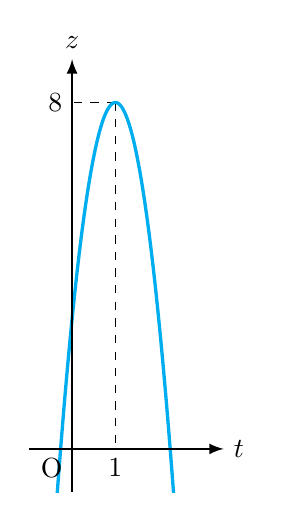
\begin{tikzpicture}[scale=0.55,samples=300]
            \draw [dashed] (1,8) -- (1,0) node [below] {$1$};
            \draw [dashed] (1,8) -- (0,8) node [left] {$8$};
            \begin{scope}
              \clip(-1,-1) rectangle(3,9);
              \draw [smooth,very thick,cyan] plot (\x,-5*\x*\x+10*\x+3);
            \end{scope}
            \draw [-latex,thick] (-1,0) -- (3.5,0) node [right]{$t$};
            \draw [-latex,thick] (0,-1) -- (0,9) node [above]{$z$};
            \draw (0,0) node [below left] {O};
          \end{tikzpicture}
        \caption{$z$座標と時間の変化}
        \end{wrapfigure}

        \begin{equation}
        \renewcommand{\arraystretch}{2}
        \begin{array}{rcl}
          z(t)
          &=&
          −5t^2 + 10t + 3
          \\
          &=&
          −5\left(t^2 + \dfrac{10t}{−5}\right) + 3
          \\
          &=&
          −5(t^2 − 2t) + 3
          \\
          &=&
          −5(t^2 − 2t + 1^2 − 1^2) + 3
          \\
          &=&
          −5(t − 1)^2 + (−5 \cdot −1) + 3
          \\
          &=&
          −5(t − 1)^2 + 8\ \cdots\ 平方完成
        \end{array}
      \end{equation}
      \begin{center}
        $\therefore\ t=1$\ のとき\ $z_{\mathrm{max}}=8$
      \end{center}
    \end{minipage}

    \vs{10}

      \begin{equation}
        \renewcommand{\arraystretch}{2}
        \begin{array}{rcl}
          \bm{r}(1)
          &=&
          (2t+1 \quad 1 \quad -5t^{2}+10t+3) \ \cdots (\ast)
          \\
          &=&
          ((2 \times 1)+1 \quad 1 \quad (-5 \times 1)^{2}+(10 \times 1)+3)
          \\
          &=&
          (3 \quad 1 \quad 8)
          \\
        \end{array}
      \end{equation}

      \item 別解（最高点のとき速度$0$になることを利用．）
      \begin{equation}
        \renewcommand{\arraystretch}{2}
        \begin{array}{rcl}
          \dot{\bm{r}}(t)
          &=&
          \bm{0}
          \\
          \dot{z}(t)
          &=&
          -10t+10 =0
          \\
          &\Leftrightarrow&
          t=1\ \cdots あとは\ (\ast)\ の計算へ移動
          \\
        \end{array}
      \end{equation}
    \end{itemize}
  \end{enumerate}

\subsection{直線の運動方程式}

世の中の物体を考えると基本的には移動だけである．
移動を考える中で物体の大きさを考えると複雑化してしまうので，便宜上一点のみを考える．
この点のことを質点と呼ぶ．

\subsubsection{運動方程式の立て方}

\begin{enumerate}
  \item 物体の運動（\textbf{物体間の力}（垂直抗力を忘れずに）と\textbf{重力のベクトル}）を図示する．
  \item 初期条件（\textbf{初速度}と\textbf{初期地}）を座標で示す．
  \item どのベクトルが釣り合っているのか否か調べ，釣り合っていないベクトルを$\bm{F}$として$m\ddot{x}=\bm{F}$に代入する．
  \begin{itemize}
    \item $x$軸方向は必ず\textbf{等速直線運動}するため，\colorbox{yellow}{$加速度\ \ddot{x}(t) = 0$}である．
    \item $y$軸方向は必ず\textbf{自由落下}するため，\colorbox{yellow}{$加速度\ \ddot{y}(t) = -g$}
  \end{itemize}
  \item 立てた運動方程式を微分方程式とみなし計算する．
\end{enumerate}

\clearpage

\subsubsection{運動方程式を解くと公式になる}

よく講義内で「へんな公式」という言葉が多用されている．しかし，運動方程式を解くと一般に知られている
公式になるので共有しておく．
問題を解くうえでは，運動方程式を立てた後に公式代入し同値変換したかのように見せるのが楽だろう．

\begin{equation}
  \renewcommand{\arraystretch}{2}
  \begin{array}{rl}
    &\ m \ddot{x} = \bm{F}
    \\
    \Leftrightarrow
    &\ \ddot{x} = \dfrac{\bm{F}}{m}
    \\
    \Leftrightarrow
    &\ \dot{x} = At + B\ \cdots\ (\ast)
    \\
    \Leftrightarrow
    &\ x = \dfrac{1}{2}At^{2} + Bt + C\ \cdots\ (\ast \ast)
  \end{array}
\end{equation}

$(\ast)$ の式に対してみると，

\begin{equation}
  \renewcommand{\arraystretch}{2}
  \begin{array}{rl}
    &\ \dot{x} = At + B
    \\
    \Leftrightarrow
    &\ \bm{v} = \bm{a}t + \bm{v}_{0}
    \\
  \end{array}
\end{equation}

$(\ast \ast)$ の式に対してみると，

\begin{equation}
  \renewcommand{\arraystretch}{2.5}
  \begin{array}{rl}
    &\ x = \dfrac{1}{2}At^{2} + Bt + C
    \\
    \Leftrightarrow
    &\ \bm{r} = \dfrac{1}{2}\bm{a}t^{2} + \bm{v}_{0}t + x_{0}
    \\
  \end{array}
\end{equation}

これらのことから，

\begin{table}[hb]
  \centering
  \begin{tabular}{cc}
    (左辺) =
    $
    \begin{cases}
      \ddot{x} = \bm{a} \\
      \dot{x} = \bm{v} \\
      x = \bm{r} \\
    \end{cases}
    $
    &
    $
    (右辺) =
    \begin{cases}
      A = \bm{a} \\
      B = \bm{v}_{0} \\
      C = \bm{r}_{0}
    \end{cases}
    $
  \end{tabular}
\end{table}

と記述できるため，そもそも微分方程式を解いたらいわゆる「へんな公式」になる．

\clearpage

\subsection{第5回\ 問題演習}

\begin{enumerate}
  \item 質量$m=10$\ [kg]の小さな物体が，水平と角度20度をなす粗い斜面上に止まっている．物体に働く垂直抗力の大きさを答えよ．
  \begin{table}[hb]
    \centering
    \begin{tabular}{rcccccc}
      $\bm{G}$ & $=$ & ( & $mg \sin 20^{\circ}$ & $-mg \cos 20^{\circ}$ & ) \\
      $\bm{N}$ & $=$ & ( & $0$ & $N$ & ) \\
      $+\ )\ \bm{F}$ & $=$ & ( & $-F$ & $0$ & ) \\
    \hline
      $\bm{G}+\bm{N}+\bm{F}$ & $=$ & ( & $mg \sin 20^{\circ}-F$ & $N-mg \cos 20^{\circ}$ & ) \\
    \end{tabular}
  \end{table}

  斜面上に静止しているため，$\ddot{x}=0$ である．そのため，$(合力) = 0$ となる．
  題意に則すと，$\bm{G}+\bm{N}+\bm{F} = \bm{0}$ となるので次のような連立方程式が立てられる．

  \begin{equation}
    \renewcommand{\arraystretch}{2}
    \begin{array}{rcl}
      \begin{cases}
        mg \sin 20^{\circ}-F = 0 \\
        N-mg \cos 20^{\circ} = 0
      \end{cases}
      &\Leftrightarrow&
      \begin{cases}
        F = mg \sin 20^{\circ} \\
        N = mg \cos 20^{\circ}
      \end{cases} \\
      \\[-20pt]
      &\Leftrightarrow&
      \begin{cases}
        F = 10 \times 9.8 \times 0.34 \\
        N = 10 \times 9.8 \times 0.94
      \end{cases} \\
      \\[-20pt]
      &\Leftrightarrow&
      \begin{cases}
        F = 33.32 \\
        N = 92.12
      \end{cases} \\
    \end{array}
  \end{equation}

  垂直抗力は重力の反作用にあたるため，$N \simeq 92$ [N]となる．

\hs{0}

  \item[\textbf{別解？}] 重力の反作用が垂直抗力のため，$N = mg \cos 20^{\circ}$ [N] と記述できる．

\end{enumerate}

\clearpage

\subsection{第6回\ 問題演習}

\begin{enumerate}
  \item 地面に固定された滑らかな水平面に，質量$3.5$\ [kg]の物体が止まっている．この物体を，水平面に平行な一定方向に，大きさ$14$\ [kg \cdot m/$\mathrm{sec}^{2}$]の力で押し続けた．
  \begin{itemize}
    \begin{equation}
      \renewcommand{\arraystretch}{2}
      \begin{array}{rl}
        &\ m \ddot{x} = \bm{F}
        \\
        \Leftrightarrow
        &\ 3.5 \ddot{x}(t) = 14
        \\
        \Leftrightarrow
        &\ \dot{x}(t) = At + B
        \\
        \Leftrightarrow
        &\ x(t) = 2t^{2} + Ct + D
        \\
      \end{array}
    \end{equation}
    初期条件より，
    $
    \begin{cases}
      x(0)=0 \\
      \dot{x}(0)=0
    \end{cases}
    $
    となる．\\
\vs{10}
    初期条件を考慮に入れると，
    $
    \begin{cases}
      距離\ x(t)=2t^{2} \\
      速度\ \dot{x}(t)=4t
    \end{cases}
    $ となる． 
\vs{10}
    \item 押し始めてから$3.0$秒後の物体の位置と速さを答えよ．
\vs{10}

    時刻 $t=3$ より，
    $
    \begin{cases}
      距離\ x(3)=2 \times 3^{2} = 18 \\
      速度\ \dot{x}(3) = 4 \times 3 =12
    \end{cases}
    $ となる．

\vs{10}

\begin{center}
  \therefore\ 元の位置から力の方向に，$18$\ [m] の位置で $12$\ [m/s] の速さで運動する．
\end{center}

\vs{10}
    \item 物体の速さが$20$\ [m/s]になる瞬間はいつか答えよ．
\vs{10}
    
    速さが $20$\ [m/s] より，
    \begin{equation}
      \renewcommand{\arraystretch}{2}
      \begin{array}{rl}
        &\ |\dot{x}(t)| = 4t
        \\
        \Leftrightarrow
        &\ 4t = 20
        \\
        \Leftrightarrow
        &\ t = 5
        \\
      \end{array}
    \end{equation}

\begin{center}
  \therefore\ 押し始めてから $5$秒後に物体の速さが$20$\ [m/s] になる．
\end{center}
    
\clearpage

    \item 物体が距離$32$\ [m]進んだ瞬間の速さを答えよ．
    \vs{10}

    距離が $32$\ [m/s] より，

    \begin{equation}
      \renewcommand{\arraystretch}{2}
      \begin{array}{rccl}
        位置
        &
        x(t)
        &=&
        32
        \\
        \Leftrightarrow
        &
        2t^{2}
        &=&
        32
        \\
        \Leftrightarrow
        &
        t
        &=&
        4
        \\
        速さ
        &
        |\dot{x}(4)|
        &=&
        4 \times 4
        \\
        &
        &=&
        16
      \end{array}
    \end{equation}

\begin{center}
  \therefore\ 瞬間の速さが $16$\ [m/s] のとき，物体が $32$\ [m] 進んだ．
\end{center}

  \end{itemize}
\end{enumerate}

\subsection{第7回\ 問題演習}

\begin{enumerate}
  \item 天井に糸で吊るされた質量 $m=4$\ [kg] のおもりが，手で水平方向に $37^{\circ}$ 押されて，静止している，手で押している力 $\bm{F}$ の大きさ $F$ を数値と適切な単位で答えなさい．\\
  なお，$\sin 37^{\circ}=\dfrac{3}{5}$，$\cos 37^{\circ}=\dfrac{4}{5}$，$\tan 37^{\circ}=\dfrac{3}{4}$ とする．
  \begin{table}[hb]
    \centering
    \begin{tabular}{rcccccc}
      $\bm{F}$ & $=$ & ( & $F$ & $0$ & ) \\
      $\bm{G}$ & $=$ & ( & $0$ & $-mg$ & ) \\
      $+\ )\ \bm{T}$ & $=$ & ( & $-T \sin 37^{\circ}$ & $T \cos 37^{\circ}$ & ) \\
    \hline
      $\bm{F}+\bm{G}+\bm{T}$ & $=$ & ( & $F-T \sin 37^{\circ}$ & $-mg+T \cos 37^{\circ}$ & ) \\
    \end{tabular}
  \end{table}

題意より，$\bm{F}+\bm{G}+\bm{T} = \bm{0}$ となるので次のような連立方程式が立てられる．

  \begin{equation}
    \renewcommand{\arraystretch}{2}
    \begin{array}{rcl}
      \begin{cases}
        F-T \sin 37^{\circ} = 0 \\
        -mg+T \cos 37^{\circ} = 0
      \end{cases}
      &\Leftrightarrow&
      \begin{cases}
        F-\dfrac{3}{5}T = 0 \\
        -mg+\dfrac{4}{5}T = 0
      \end{cases}
      \\[20pt]
      &\Leftrightarrow&
      \begin{cases}
        5F - 3T = 0 \\
        -196 + 4T = 0
      \end{cases}
      \\[10pt]
      &\Leftrightarrow&
      \begin{cases}
        T = 49 \\
        F = 29.4
      \end{cases}
    \end{array}
  \end{equation}

\begin{center}
  力 $\bm{F}$ の大きさ $F$ を求めればよいので，$F = 29.4$ [kg \cdot m/$\mathrm{s}^2$]となる．
\end{center}

\clearpage

  \item 地面のある地点からある時刻に，質量 $m=200$\ [g] のボールを，水平から角度 $30^{\circ}$ の方向に速さ $\bm{v}_{0} = 19.6$\ [m/s] で打ち出す．空気抵抗は無視しても良い．重力加速度は $\bm{g} = 9.8$\ [m/$\mathrm{s}^{2}$] とする．

\vs{11}
  \begin{itemize}
    \item 座標系を設定し，ボールの運動方程式を立てなさい．\\

\vs{-11}
    運動方程式 $m \ddot{\bm{r}} = -m\bm{g} \bm{j}$ より，
    \begin{equation}
      m(\ddot{x}(t) \quad \ddot{y}(t))=(0 \quad -mg)
    \end{equation}
    \item 運動方程式を解いて，ボールの運動を求めなさい．

\vs{11}
    \begin{table}[hb]
      \centering
      \begin{tabular}{lcl}
        $x$ について，$m \ddot{x}(t) = 0$ より， & & $y$ について，$m \ddot{y}(t) = -mg$ より， \\
        $
        \renewcommand{\arraystretch}{2}
        \begin{array}{rl}
          &\ddot{x}(t)=0
          \\
          \Leftrightarrow
          & \dot{x}(t) = A
          \\
          \Leftrightarrow
          & x(t) = At+B
        \end{array}
        $
        & &
        $
        \renewcommand{\arraystretch}{2}
        \begin{array}{rl}
          &\ddot{y}(t)=-g
          \\
          \Leftrightarrow
          & \dot{y}(t) = -gt+C
          \\
          \Leftrightarrow
          & y(t) = - \dfrac{1}{2}gt^{2}+Ct+D
        \end{array}
        $ \\ \\
        初期条件より， & & 初期条件より，\\[11pt]
        $
        \begin{cases}
          x(0)=0 \\
          \dot{x}(0)=19.6 \cos 30^{\circ}
        \end{cases}
        $
        & &
        $
        \begin{cases}
          y(0)=0 \\
          \dot{y}(0)=19.6 \sin 30^{\circ}
        \end{cases}
        $
      \end{tabular}
    \end{table}

\vs{11}
    \item ボールが地面に戻る時刻とその地点を答えなさい．
    
\vs{11}
    ボールが地面に戻る時間は，$y(t)=0$ より，
    \begin{equation}
      0=-\dfrac{1}{2}gt^{2}+Ct+D
    \end{equation}

    初期条件を考慮に入れると，
    \begin{equation}
      \renewcommand{\arraystretch}{2}
      \begin{array}{rl}
        & 0=-\dfrac{1}{2} \times 9.8t^{2}+19.6 \times \dfrac{1}{2}t
        \\
        \Leftrightarrow
        & 0=-4.9t^{2}+9.8t
        \\
        \Leftrightarrow
        & t=2
        \\
        \therefore
        & x(2)=19.6 \sqrt{3}
      \end{array}
    \end{equation}

  \clearpage

    \item ボールの最高点の高さを答えなさい．
    
\vs{11}
    ボールが最高点に到達するまでの時間は，戻ってくるまでの時間の半分なので1秒となる．
    \begin{equation}
      \renewcommand{\arraystretch}{2}
      \begin{array}{rcl}
        \therefore\ y(1)
        &=&
        -\dfrac{1}{2} \times 9.8 \times 1^{2} + 19.6 \times \dfrac{1}{2} \times 1
        \\
        &=&
        4.9
      \end{array}
    \end{equation}
  \end{itemize}

  \item 粗い水平面を運動する質量 $m$ の物体がある．面と物体との動摩擦係数は $\mu = 0.25$ である．物体の速さ $\bm{v}_{0}=7.0$\ [m/s] で打ち出したとき，止まるまでに面を進む距離 $L$ を求めよ．\\[-10pt]
  \item[HINT] 動摩擦係数の大きさは $\bm{F}=\mu \bm{N}=\mu m\bm{g}$ である．方向は運動と逆．進んだ距離は止まった時（速度がゼロになった時）の位置から求まる．

\vs{11}
    運動方程式 $m \ddot{x}=-\mu mg$ より，
    \begin{equation}
      \renewcommand{\arraystretch}{2}
      \begin{array}{rl}
        & \ddot{x}(t) = - \mu g
        \\
        \Leftrightarrow
        & \dot{x}(t) = - \mu gt + E
        \\
        \Leftrightarrow
        & x(t) = -\dfrac{1}{2}gt^{2}+Et+F
      \end{array}
    \end{equation}
    初期条件より，
    $
    \begin{cases}
      \mu = 0.25 \\
      E = 7.0 \\
      F = 0
    \end{cases}
    $
    となる．
    初期条件を考慮に入れると，
    \begin{equation}
      \renewcommand{\arraystretch}{2}
      \begin{array}{rl}
        & 0= - \mu gt + E
        \\
        \Leftrightarrow
        & t= \dfrac{E}{\mu g}
      \end{array}
    \end{equation}
    $L = x \left(\dfrac{E}{\mu g}\right)$ となるので，
    \begin{equation}
      \renewcommand{\arraystretch}{2.5}
      \begin{array}{rcl}
        x \left(\dfrac{E}{\mu g}\right)
        &=&
        -\dfrac{1}{2} \mu g \left(\dfrac{E}{\mu g}\right)^{2} + E \times \dfrac{E}{\mu g}
        \\
        &=& -\dfrac{1}{2} \cdot \dfrac{E^{2}}{\mu g} + \dfrac{E^{2}}{\mu g}
        \\
        &=& \dfrac{1}{2} \cdot \dfrac{E^{2}}{\mu g}
      \end{array}
    \end{equation}

    数値を代入すると，
    \begin{equation}
      \renewcommand{\arraystretch}{2.5}
      \begin{array}{rcl}
        L
        &=&
        \dfrac{1}{2} \times \dfrac{(7.0)^2}{0.25 \times 9.8}
        \\
        &=&
        \dfrac{1}{2} \times \dfrac{49}{2.45}
        \\
        &=&
        \dfrac{49}{4.9}
        \\
        &=&
        10
      \end{array}
    \end{equation}

    \begin{center}
      \therefore\ 止まるまでに面を進む距離$L$は10\ [m]である．
    \end{center}

\end{enumerate}

\clearpage

\subsection{円の運動方程式}

今までは直線に対しての運動方程式を扱ってきた．これが円になっただけである．
この円運動は，化学概論Iのボーアの水素原子モデルでも利用される．
円の運動方程式と水素原子モデルについて扱うことにする．

  \begin{wrapfigure}[13]{r}{0.26\textwidth}
  \centering
    \begin{tikzpicture}
      \def\R{1.8}
      \def\ang{43}
      \coordinate (O) at (0,0);
      \coordinate (X) at (2,0);
      \coordinate (R) at (\ang:\R);
      \filldraw (O) circle (1.5pt);
      \draw[dashed] (0,0) -- (\R,0);
      \draw[-latex,very thick,orange] (O) -- (R) node[below right] at ($(O)!0.7!(R)$) {$\bm{r}$};
      \draw pic["$\theta$",draw=black,angle radius=15,angle eccentricity=1.5] {angle=X--O--R};
      \draw[-Stealth,thick,magenta] (\ang+30:0.6*\R) arc(\ang+20:\ang+70:0.4*\R) node[midway,above] {$\omega$};
      \draw[thick] (O) circle (\R);
      \draw[-latex,very thick,cyan] (R) --++ (\ang+90:1) node[above left] {$\bm{v}$};
      \filldraw (R) circle (3pt);
    \end{tikzpicture}
  \caption{円運動ではたらく力}
  \end{wrapfigure}

等速円運動では，回転中心の周りの角$\theta$\ [rad]を時間$t$\ [s]の一次函数として，

\begin{equation}
  \theta_0 = \omega_0 t + \theta_0
\end{equation}

と表せる．このとき{\color{magenta} $\omega$は角速度}，$\theta$は周りの角のため，$\omega_0$は初期の角速度，$\theta_0$は初期の角度であり定数（const.）である．

運動方程式は，{\color{orange} 位置ベクトル$\bm{r}$}を微分して求められる．位置ベクトル$\bm{r}$は，

\begin{equation}
  \bm{r} = (r\cos\theta \quad r\sin\theta)
\end{equation}

$\theta$は上記で$\omega_0 t + \theta_0$と分かっているので，$\theta$に$\theta_0$を代入すると

\begin{equation}
  \bm{r} = \Big(r\cos(\omega_0 t + \theta_0) \quad r\sin(\omega_0 t + \theta_0)\Big)
\end{equation}

と示される．ここから微分をして速度函数や加速度函数を求めることができる．
三角函数（$\sin$，$\cos$）は微分すると位相が$90^\circ$ズレることを考慮に入れ計算すると，

\begin{equation}
  \begin{array}{rccr}
    {\color{cyan} \dot{\bm{r}}} &=& \Big(-r\omega_0 \sin(\omega_0 t + \theta_0) & r\omega_0 \cos(\omega_0 t + \theta_0)\Big) \\[10pt]
    \ddot{\bm{r}} &=& \Big(-r\omega^2_0 \cos(\omega_0 t + \theta_0) & -r\omega^2_0 \sin(\omega_0 t + \theta_0)\Big)
  \end{array}
\end{equation}

となる．これらの式から言えることは，三角函数を噛ますと直線の運動方程式よりも簡易な式で位置，速度，加速度を表せる．

\begin{equation}
  \ddot{\bm{r}}(t) = -\omega^2_0 {\color{cyan}\dot{\bm{r}}(t)}
\end{equation}

この式が表していることは，{\color{cyan} 速度$\bm{v}$}に$\omega^2$を掛けると加速度の大きさ$\bm{a}$となる．

上記同様に{\color{orange} 位置 \bm{r}}と{\color{cyan} 速度 \bm{v}}にも次の関係が成り立つ．

\begin{equation}
  {\color{cyan} \dot{\bm{r}}} = {\color{orange}r}\omega_0
\end{equation}

{\color{orange} 位置$\bm{r}$}に$\omega$を掛けると{\color{cyan} 速度$\bm{v}$}，{\color{cyan} 速度$\bm{v}$}に$\omega$を掛けると加速度の大きさ$\bm{a}$と簡単に記述できる．

\clearpage

\subsection{ボーアの水素原子モデル}

ボーアが考えた原子モデルは，惑星軌道と似た形をしている．この際，原点が陽子，円運動する物体が電子である．また，原子核である陽子と中性子を構成するものをクォーク（quark），陽子のことをプロトン（proton），電子のことをレプトン（lepton）と呼ぶ．

まず，物体間の力（非接触力（万有引力，静電気力，磁力のこと））は逆2乗則によって記述される．

\begin{wrapfigure}[7]{r}{0.4\textwidth}
\centering
\begin{tikzpicture}[scale=1.2]
  \def\d{4.1}  % distance r
  \def\r{0.3}  % small radius ball
  \def\R{0.38} % large radius ball
  \def\F{0.95} % -Stealth,orange,thick,line cap=round magnitude
  \def\u{0.4}  % unit vector magnitude
  \def\ang{5}  % angle lin
  \coordinate (M1) at (0,0);
  \coordinate (M2) at (\ang:\d);
  
  % SETUP
  \draw[cyan]
    (M1) --++ (\ang+90:1.6*\R)
    (M2) --++ (\ang+90:1.6*\R);
  \draw[latex-latex,cyan] ($(M1)+(\ang+90:1.35*\R)$) --++ (M2)
    node[midway,circle,fill=white,inner sep=0] {$r$};
  \draw[dashed] (M1) -- (M2);
  \draw[red!30!black,fill=red!40!black!10,rounded corners=1,top color=red!40!black!20,bottom color=red!40!black!10,shading angle=20] (M1) circle(\r) node[scale=0.9] {\footnotesize $m_1$};
  \draw[semithick,red!30!black,fill=red!40!black!10,rounded corners=1,top color=red!40!black!20,bottom color=red!40!black!10,shading angle=20] (M2) circle(\R) node[scale=0.9] {$m_2$};
  
  % -Stealth,orange,thick,line cap=roundS
  \draw[-Stealth,orange,thick,line cap=round] (M1)++(\ang-8:0.9*\r) --++ (\ang:\F)
    node[anchor=90,inner sep=4] {$\bm{F}$}; % = -G\dfrac{m_1m_2}{r^2}\vu{r}_{21}
  \draw[-Stealth,orange,thick,line cap=round] (M2)++(\ang-172:0.9*\R) --++ (\ang:-\F)
    node[anchor=130,inner sep=3] {$\bm{F}$}; % = -G\dfrac{m_1m_2}{r^2}\vu{r}_{12}
  
\end{tikzpicture}
\caption{2物体間にはたらく力}
\end{wrapfigure}

2つの物体があるときに働く力$\bm{F}$は，2つの質量$m_1$，$m_2$と距離$r$の2乗の比で求められる．数式では，

\begin{equation}
  \bm{F} = G \dfrac{m_1 m_2}{\bm{r}^2}
\end{equation}

と表現される．このときの$G$は，万有引力定数であり$0.67 \times 10^{-11}\ [\mathrm{N \cdot m^2 / kg}]$である．

\begin{wrapfigure}[11]{l}{0.36\textwidth}
\centering
\begin{tikzpicture}[scale=1.5]
  \tikzset{fieldlines/.style={orange,decoration={markings,mark=at position #1 with {\arrow{latex}}},
                            postaction={decorate},line width=0.7},
         fieldlines/.default=0.55}
  \def\W{2.4}   % preaction={fill,top color=black!10,bottom color=black!5,shading angle=20},                     fill,pattern=north east lines,draw=none,minimum width=0.3,minimum height=0.6 width
  \def\D{0.2}   % preaction={fill,top color=black!10,bottom color=black!5,shading angle=20},                     fill,pattern=north east lines,draw=none,minimum width=0.3,minimum height=0.6 depth
  \def\H{1.5}   % height
  \def\E{0.35}  % Earth's radius
  \def\R{1.3}   % field line max. radius
  \def\N{10}    % number of field lines
  \def\rang{45} % angle or r axis
  
  % FIELD LINES
  \foreach \i [evaluate={\ang=\i*360/\N;}] in {1,...,\N}{
    \draw[fieldlines=0.6] (\ang:\R) -- (\ang:\E); % field lines
  }
  
  % EARTH
  \fill[blue!70!black!70] (0,0) circle(\E);
  \begin{scope}[rotate=-11]
    \clip (0,0) circle(\E);
    \fill[white] (0,\E) ellipse({0.6*\E} and {0.15*\E});
    \fill[white] (0,-\E) ellipse({0.8*\E} and {0.08*\E});
    \fill[green!70!black!60,rotate=-30] (160:1.1*\E) ellipse({0.2*\E} and {0.8*\E});
    \fill[green!70!black!60,rotate=40] (-10:1.14*\E) ellipse({0.2*\E} and {0.9*\E});
    \fill[green!60!black!60,very thick,rotate=-20] % Australia
      (230:0.86*\E) ellipse({0.25*\E} and {0.18*\E});
  \end{scope}
  \draw[line width=0.3] (0,0) circle(\E);
  
\end{tikzpicture}
\caption{地球全体にはたらく力}
\end{wrapfigure}

また，この$G$は$\dfrac{1}{4\pi k_0}$と記述でき分母に$4\pi r^2$が出てくる．
これは球の表面積の一致しており，地球に一様の力が掛かっていることを数式的にも表現されている．

また，静電気力の逆2乗則は次のように書き換えられる．

\begin{equation}
  \bm{F} = k_e \dfrac{q_1 \times q_2}{|\bm{r}_2 - \bm{r}_1|^2} \times \dfrac{\bm{r}_2 - \bm{r}_1}{|\bm{r}_2 - \bm{r}_1|}
\end{equation}

このとき$k_e$が定数，$q_1 \times q_2$が電荷，$|\bm{r}_2 - \bm{r}_1|^2$が逆2乗則，$\dfrac{\bm{r}_2 - \bm{r}_1}{|\bm{r}_2 - \bm{r}_1|}$が単位ベクトル（方向づけ）である．
このようにベクトルとして表現され，原子の運動も同じである．

  \begin{wrapfigure}[15]{r}{0.36\textwidth}
  \centering
  \vs{10}
    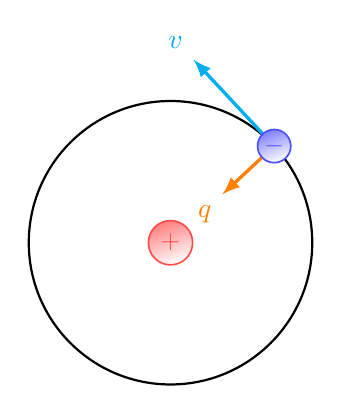
\begin{tikzpicture}
      \def\R{1.8}
      \def\ang{43}
      \coordinate (O) at (0,0);
      \coordinate (X) at (2,0);
      \coordinate (R) at (\ang:\R);
      \filldraw (O) circle (1.5pt);
      \draw[thick] (O) circle (\R);
      \draw[-latex,very thick,cyan] (R) --++ (\ang+90:1.5) node[above left] {$\bm{v}$};
      \draw[-latex,very thick,orange] (R) --++ (\ang+180:0.9) node[below left] {$\bm{q}$};
      \draw[semithick,blue!70!white,bottom color=white,top color=blue!50!white,shading angle=20] (R) circle(6pt) node[scale=0.9] {$-$};
      \draw[semithick,red!70!white,bottom color=white,top color=red!50!white,shading angle=20] (0,0) circle(8pt) node[scale=0.9] {$+$};
    \end{tikzpicture}
  \caption{ボーアの模型ではたらく力}
  \end{wrapfigure}

それでは本題に入る．陽子と電子には引力がはたらく．この引力（クーロン力）は向心力と同じであるため，次の等式が成り立つ．

\begin{equation}
  m\dfrac{\bm{v}^2}{\bm{r}} = k_0\dfrac{\bm{e}^2}{\bm{r}^2}
\end{equation}

また，ボーアの量子条件として電子は原子核の周囲を\textbf{等速円運動}しており，
電子の質量を$m$\ [kg]，その速度の大きさを$\bm{v}$\ [m/s]，回転の軌道半径を$r$\ [m]，
プランク定数$h$\ [J \cdot s]として，$n \in \mathbb{N}$\footnote{$n$は
$\mathbb{N}（自然数）$であるという意．}とするとき，次の関係が成立する．

\begin{equation}
  m\bm{v}r = n \cdot \dfrac{h}{2\pi}（n \in \mathbb{N}）
\end{equation}                                                    

\clearpage

\subsection{波の性質}

円運動と波は密接に関わっている．円運動を正射影すると単振動になり，それを縦軸に高さ$y$，横軸に時間$t$の$y-t$グラフにするとサインカーブ（正弦波）を描く．

\begin{figure}[h]
  \centering
  \def\xmax{6.6} % max x axis
  \def\ymax{1.2} % max y axis
  \def\A{0.8}    % amplitude
  \begin{tikzpicture}[samples=\N,scale=2]
  % AXIS
    \draw[-latex,thick] (0,-\ymax) -- (0,\ymax) node[above] {$y$};
    \draw[-latex,thick] (-0.2*\ymax,0) -- (\xmax,0) node[right] {$t$\ [s]};
    \draw[dashed] ({360/(2.55*360/(0.94*\xmax))},1.2*\A) --++ (0,-2.7*\A);
    \tick{0,\A}{0} node[left] {$A$};
    \tick{{360/(2.55*360/(0.94*\xmax))},0}{90} node[below,scale=0.9] {\colorbox{white}{$T$}};
    \tick{{720/(2.55*360/(0.94*\xmax))},0}{90} node[below,scale=0.9] {$2T$};
    \draw[Stealth-Stealth] (0,-1.35*\A) --++ ({360/(2.55*360/(0.94*\xmax))},0) node[midway,fill=white,inner sep=1,scale=0.9] {$T = \dfrac{2\pi}{\omega}$};
  % PLOT
    \draw[cyan,very thick,smooth,variable=\x,domain=0:0.94*\xmax] plot(\x,{\A*cos((2.55*360/(0.94*\xmax))*\x)});
  \end{tikzpicture}
  \caption{正弦曲線（$y-t$グラフ）}
\end{figure}

それぞれの言葉の説明を次に列挙する．

\begin{description}
  \item[波速$\bm{v}$\ \textrm{[m/s]}：] 波が媒体中を進む速さのこと．
  \item[波長$\lambda$\ \textrm{[m]}：] 山1つ谷1つ，または山頂から次の山頂まで，谷底から次の谷底までの長さのこと．
  \item[回転数$f$\ \textrm{[Hz]}：] 単位時間あたりに円をまわる回数．グラフ上では単位時間の波長数のこと．
  \item[周期$T$\ \textrm{[s]}：] 波が1往復するのにかかる時間のこと．$T^{-1}\ [s^{-1}] = \lambda$\ [Hz]．
  \item[振幅$A$\ \textrm{[m]}：] 振動の大きさ（準線からピーク）のこと．山頂から谷底までの長さの\textbf{2分の1}であることに注意．
\end{description}

\clearpage

\subsection{第10回\ 問題演習}

\begin{enumerate}
  \item 半径2.0\ [m]の円周上を5.0\ [sec]の間に20回転の等速円運動している質点がある．
        この円運動の，1秒あたりの回転数，周期，角速度，速さ，加速度の大きさを答えよ．

  \begin{center}
    題意より，回転数$n=20$\ [times]，半径$r=2.0$\ [m]，時間$t=5.0$\ [sec]と分かる．
  \end{center}

\renewcommand{\arraystretch}{2.5}
\begin{table}[h]
  \centering
  \begin{tabular}{cl}
    \textbf{1秒あたりの回転数} & $f = \dfrac{n}{t} = \dfrac{20}{5.0} = 4.0$\ [Hz] \\
    \textbf{周期}   & $T = \dfrac{1}{f} = \dfrac{5.0}{20} = 0.25$\ [sec] \\
    \textbf{角速度} & $\omega = \dfrac{2\pi}{T} = 2\pi f = 8\pi$\ [rad/s] \\
    \textbf{速さ}   & $v = r\omega = \dfrac{2\pi r}{T} = 16\pi$\ [m/s] \\
    \textbf{加速度の大きさ} & $a = v\omega = 128\pi^2$\ [$\mathrm{m/s^2}$]
  \end{tabular}
\end{table}

  \item 平面を運動する質点の位置ベクトル$\bm{r}$が，時刻$t$の函数として，次である．
  \begin{equation}
    \bm{r}(t) = \Bigg(2\cos\dfrac{\pi}{3}t \quad 2\sin\dfrac{\pi}{3}t\Bigg)
  \end{equation}
  長さ，時間，角度の単位は，左から順にmeter\ [m]，second\ [s]，radian\ [rad]である．

  \hs{0}

  \begin{enumerate}[label=\roman*.]
    \item 時刻$t=3$\ [s]での，質点の位置，速度，速さ，加速度を答えよ．
    \item[HINT] $\sin(\omega t)^{\prime} = \omega \cos(\omega t)$，$\cos(\omega t)^{\prime} = -\omega \sin(\omega t)$．
    
    \hs{0}

    まず，時刻$t=3$での質点の位置は，題意の式にそのまま代入するだけである．

    \begin{equation}
      \begin{array}{rcl}
        \bm{r}(3) &=& \Bigg(2\cos\left(\dfrac{\pi}{3} \times 3\right) \quad 2\sin\left(\dfrac{\pi}{3} \times 3\right)\Bigg) \\
        &=& (2 \cdot -1 \quad 2 \cdot 0) \\
        &=& (-2 \quad 0)
      \end{array}
    \end{equation}

\clearpage

    質点の速度は質点の位置を1階微分して$t=3$を代入する．そして絶対値を取り速さを求める．

    \vs{-10}

    \renewcommand{\arraystretch}{3.5}
    \begin{equation}
      \begin{array}{rcl}
        \dot{\bm{r}}(t) &=& \Bigg(\left(2\cos\dfrac{\pi}{3}t\right)^{\prime} \quad \left(2\sin\dfrac{\pi}{3}t\right)^{\prime}\Bigg) \\
        &=& \Bigg(-2 \cdot \dfrac{\pi}{3}\sin\dfrac{\pi}{3}t \quad 2 \cdot \dfrac{\pi}{3}\cos\dfrac{\pi}{3}t\Bigg) \\
        \dot{\bm{r}}(3) &=& \Bigg(-2 \cdot \dfrac{\pi}{3}\sin\left(\dfrac{\pi}{3} \times 3\right) \quad 2 \cdot \dfrac{\pi}{3}\cos\left(\dfrac{\pi}{3} \times 3\right)\Bigg) \\
        &=& \Bigg(-2 \cdot \dfrac{\pi}{3} \cdot 0 \quad 2 \cdot \dfrac{\pi}{3} \cdot -1\Bigg) \\
        &=& \Bigg(0 \quad -\dfrac{2}{3}\pi\Bigg) \\
        |\dot{\bm{r}}(3)| &=& \sqrt{0^2 + \left(-\dfrac{2}{3}\pi\right)^2} \\
        &=& \dfrac{2}{3}\pi\ [\mathrm{m/s}]
      \end{array}
    \end{equation}

    質点の加速度は質点の速度を1階微分して$t=3$を代入する．

    \vs{-10}

    \renewcommand{\arraystretch}{3.5}
    \begin{equation}
      \begin{array}{rcl}
        \ddot{\bm{r}}(t) &=& \Bigg(\left(-2 \cdot \dfrac{\pi}{3}\sin\dfrac{\pi}{3}t\right)^{\prime} \quad \left(2 \cdot \dfrac{\pi}{3}\cos\dfrac{\pi}{3}t\right)^{\prime}\Bigg) \\
        &=& \Bigg(-2 \left(\dfrac{\pi}{3}\right)^2\cos\dfrac{\pi}{3}t \quad -2 \left(\dfrac{\pi}{3}\right)^2 \sin\dfrac{\pi}{3}t\Bigg) \\
        \ddot{\bm{r}}(3) &=& \Bigg(-2 \left(\dfrac{\pi}{3}\right)^2\cos\left(\dfrac{\pi}{3} \times 3\right) \quad -2 \left(\dfrac{\pi}{3}\right)^2 \sin\left(\dfrac{\pi}{3} \times 3\right)\Bigg) \\
        &=& \Bigg(-2 \cdot \left(\dfrac{\pi}{3}\right)^2 \cdot -1 \quad 2 \cdot \left(\dfrac{\pi}{3}\right)^2 \cdot 0\Bigg) \\
        &=& \Bigg(2 \left(\dfrac{\pi}{3}\right)^2 \quad 0\Bigg) \\
      \end{array}
    \end{equation}

    \clearpage

    \item 質点が描く軌跡はどのような図形か答えよ．
    \vs{10}
    \item[HINT] $t = 0,\ 1,\ 2,\ 3,\ 4,\ 5,\ 6,\ \dfrac{3}{2}$\ などで位置を求めてから滑らかに結ぶ．
    
    \vs{5}

    \begin{minipage}{\linewidth}
      \begin{wrapfigure}{r}{0.4\textwidth}
      \centering
        \begin{tikzpicture}[samples=\N]
        % AXIS
          \draw[-latex,thick] (0,-3) -- (0,3) node[above] {$y$};
          \draw[-latex,thick] (-3,0) -- (3,0) node[right] {$x$};
          \draw[cyan,very thick] (0,0) circle (2);
        % PLOT
          \fill (2,0) circle (2.5pt) node[below right] {$\bm{r}(0)$};
          \fill (1,{sqrt(3)}) circle (2.5pt) node[above right] {$\bm{r}(1)$};
          \fill (-1,{sqrt(3)}) circle (2.5pt) node[above left] {$\bm{r}(2)$};
          \fill (-2,0) circle (2.5pt) node[below left] {$\bm{r}(3)$};
          \fill (-1,-{sqrt(3)}) circle (2.5pt) node[below left] {$\bm{r}(4)$};
          \fill (1,-{sqrt(3)}) circle (2.5pt) node[below right] {$\bm{r}(5)$};
          \fill (2,0) circle (2.5pt) node[above right] {$\bm{r}(6)$};
          \fill (0,2) circle (2.5pt) node[above left] {$\bm{r}\left(\dfrac{3}{2}\right)$};
        \end{tikzpicture}
      \caption{位置函数のプロット}
      \end{wrapfigure}

      まず，速度函数は次である．

      \vs{-15}

      \begin{footnotesize}
        \begin{equation}
          \begin{array}{rcl}
          \bm{r}(t) &=& \Bigg(2\cos\left(\dfrac{\pi}{3} t\right) \quad 2\sin\left(\dfrac{\pi}{3} t\right)\Bigg)
          \end{array}
        \end{equation}
      \end{footnotesize}

      \vs{5}
  
      速度函数に$t=0$を代入すると次である．
  
      \vs{-15}

      \begin{footnotesize}
        \begin{equation}
          \begin{array}{rcl}
          \bm{r}(0) &=& \Bigg(2\cos\left(\dfrac{\pi}{3} \times 0\right) \quad 2\sin\left(\dfrac{\pi}{3} \times 0\right)\Bigg) \\
          &=& \Bigg(2\cos 0 \quad 2\sin 0\Bigg) \\
          &=& (2 \quad 0)
          \end{array}
        \end{equation}
      \end{footnotesize}

      速度函数に$t=1$を代入すると次である．
  
      \vs{-15}
  
      \begin{footnotesize}
        \begin{equation}
          \begin{array}{rcl}
          \bm{r}(1) &=& \Bigg(2\cos\left(\dfrac{\pi}{3} \times 1\right) \quad 2\sin\left(\dfrac{\pi}{3} \times 1\right)\Bigg) \\
          &=& \Bigg(2\cos\dfrac{\pi}{3} \quad 2\sin\dfrac{\pi}{3}\Bigg) \\
          &=& (1 \quad \sqrt{3})
          \end{array}
        \end{equation}
      \end{footnotesize}

    \end{minipage}

これを複数回，計算する．これの解答を記述するのは愚か，各自で計算して導くこと．
よって，原点を中心に半径2の円の軌跡を描く．$_■$

  \vs{5}

  \item[\textbf{別解？}] 三角函数の定義および円の媒介変数表示は$(\cos\theta \quad \sin\theta)$であることは既知なので，
                         原点を中心に半径2の円の軌跡を描く．
  
  \end{enumerate}
\end{enumerate}

以下に三角比表を記載しておく．必要に応じて利用すること．

\renewcommand{\arraystretch}{1.8}
\begin{table}[h]
  \centering
  \begin{tabular}{ccccccccc}
    \hline
    $\theta$\ [rad] & 0 & $\dfrac{\pi}{3}$ & $\dfrac{\pi}{2}$ & $\dfrac{2}{3}\pi$ & \pi & $\dfrac{4}{3}\pi$ & $\dfrac{5}{3}\pi$ & 2\pi \\
    \hline
    $\sin\theta$ & 0 & $\dfrac{\sqrt{3}}{2}$ & 1 & $\dfrac{\sqrt{3}}{2}$ & 0 & $-\dfrac{\sqrt{3}}{2}$ & $-\dfrac{\sqrt{3}}{2}$ & 0 \\
    $\cos\theta$ & 1 & $\dfrac{1}{2}$ & 0 & $-\dfrac{1}{2}$ & $-1$ & $-\dfrac{1}{2}$ & $\dfrac{1}{2}$ & 1 \\
    \hline
  \end{tabular}
\end{table}

\vs{-5}

  グラフをGeoGebraで作成したのでここにURLを貼り付けておきます．参考にご覧ください．

  \vs{-5}

  \begin{center}
    参考資料\ \url{https://www.geogebra.org/m/uf3kdzeq}
  \end{center}

\clearpage

\subsection{剛体による力学}

ここからは，物体の回転運動について扱う．一般に\textbf{力のモーメント}と呼ばれているが，別に物体を動かすベクトルではない．
回転させる\textbf{能力}のことである．比熱やコンデンサーのキャパシタンスと似たイメージでよい．
比熱は熱を蓄える\textbf{能力}，コンデンサーは電気を蓄える\textbf{能力}，モーメントは回転させる\textbf{能力}である．

\begin{wrapfigure}[8]{r}{0.4\textwidth}
  \centering
  \vs{-30}
    \tdplotsetmaincoords{60}{30}
      \begin{tikzpicture}[scale=2,tdplot_main_coords]
        \coordinate (O) at (0,0,0);
        \coordinate (X) at (2,0,0);
        \coordinate (Y) at (0,-1.5,0);
        \coordinate (Z) at (0,0,1.3);
        \coordinate (A) at (2,-1.5,0);
        % 地面（xy平面）の描画
        \begin{scope}[canvas is xy plane at z=0]
          \fill[cyan!30] (O) rectangle (A);
        \end{scope}
        % 3D座標軸の定義
          \draw[-latex,thick] (O) -- (Z) node[above] {$N$};
          \draw[-latex,thick] (O) -- (Y) node[below left] {$r$}; 
          \draw[-latex,thick] (O) -- (X) node[right] {$F$};
        % 地表の文字を斜めから見た感じに
          \node[canvas is xy plane at z=0] at ($(O)!0.5!(A)$) {\LARGE 面積};
          \pic[draw,canvas is xy plane at z=0,"$\theta$",-Stealth,angle radius=7mm,angle eccentricity=1.8] {angle=Y--O--X};
      \end{tikzpicture}
    \caption{位置函数のプロット}
\end{wrapfigure}

\textbf{内積}はあまり意味を持たない（仕事の計算の時にでてくるが，本質的でない）のため，次項で少ししか触れていない．
一方で，\textbf{外積}に関しては図形的意味を大きく持つので記載しておく．

外積は，

\begin{center}
  \colorbox{yellow}{2つのベクトルを張る平面に対して，} \\
  \colorbox{yellow}{垂直なベクトルを\textbf{ピンポイント}に作る．}
\end{center}

ベクトルの掛け算である．

\begin{wrapfigure}[12]{l}{0.36\textwidth}
  \centering
  \vs{-10}
          \begin{tikzpicture}[scale=0.6]
            \coordinate (O) at (1.1,0.2); % ORIGIN
            \coordinate (WT) at ( 2.9,-1.1); % WRIST TOP
            \coordinate (T1) at ( 2.3, 0.7); % THUMB
            \coordinate (T2) at ( 1.75, 2.3);
            \coordinate (T3) at ( 2.0, 3.1);
            \coordinate (T4) at (1.38, 3.15);
            \coordinate (T5) at ( 0.9, 2.3);
            \coordinate (T6) at ( 0.85, 1.2);
            \coordinate (T7) at ( 0.9, 0.2);
            \coordinate (I1) at (-0.1, 1.4); % INDEX
            \coordinate (I2) at (-1.3, 1.2);
            \coordinate (I3) at (-1.6, 0.5);
            \coordinate (I4) at (-0.7,-0.4);
            \coordinate (I5) at ( 0.1,-0.6);
            \coordinate (I6) at ( 0.1,-0.05);
            \coordinate (I7) at (-0.4,0.19);
            \coordinate (I8) at (-1.0, 0.9);
            \coordinate (M1) at (-1.8,-0.1); % MIDDLE
            %\coordinate (M2) at (-0.5,-0.7);
            \coordinate (M2) at (-0.8,-1.0);
            \coordinate (M3) at ( 0.1,-1.15);
            \coordinate (R1) at (-1.8,-0.8); % RING
            \coordinate (R2) at (-0.9,-1.6);
            \coordinate (R3) at (-0.0,-1.7);
            \coordinate (R4) at ( 0.0,-1.1);
            \coordinate (P1) at (-1.9,-1.4); % PINKY
            \coordinate (P2) at (-1.0,-2.1);
            \coordinate (P3) at (-0.3,-2.15);
            \coordinate (W1) at ( 0.4,-2.9); % WRIST BOTTOM
            \coordinate (W2) at ( 1.6,-3.5);
            
            % HAND
            \fill[pink!25]
              (WT) -- (T6) -- (I2) -- (P2) -- (W1) -- (W2) to[out=25,in=-90] cycle;
            \draw[fill=pink!25]
              (WT) to[out=120,in=-60] % THUMB
              (T1) to[out=120,in=-90]
              (T2) to[out=80,in=-110]
              (T3) to[out=80,in=50,looseness=1.5] % tip
              (T4) to[out=-130,in=80]
              (T5) to[out=-100,in=70]
              (T6) to[out=-100,in=100]
              (T7)
              (T6) -- % INDEX
              (I1) to[out=170,in=15]
              (I2) to[out=-165,in=140,looseness=1.2] % knuckle
              (I3) to[out=-60,in=140,looseness=0.8]
              (I4) to[out=-40,in=180,looseness=0.4]
              (I5) to[out=20,in=-30,looseness=1.3] % tip
              (I6) to[out=150,in=-20]
              (I7) to[out=120,in=-30]
              (I8)
              (I7) to[out=160,in=-15]++ (162:0.18)
              (I3) to[out=180,in=140,looseness=0.9] % MIDDLE
              (M1) to[out=-60,in=150,looseness=0.8]
              (M2) to[out=-30,in=175,looseness=0.4]
              (M3) to[out=-5,in=-15,looseness=1.5] % tip
              (I5)
              (M1) to[out=-130,in=135,looseness=1.2] % knuckle
              (R1) to[out=-45,in=160,looseness=0.9]
              (R2) to[out=-20,in=180,looseness=0.4]
              (R3) to[out=0,in=-15,looseness=1.5] % tip
              (M3)
              (R1) to[out=-150,in=130] % PINKY
              (P1) to[out=-50,in=165]
              (P2) to[out=-15,in=180,looseness=0.9]
              (P3) to[out=0,in=-35,looseness=1.5] % tip
              (R3)
              (P2) to[out=-35,in=145] % WRIST
              (W1) to[out=-35,in=160]
              (W2);
            
            % FOLDS
            \draw[very thin] (T5)++(-80:0.3) to[out=40,in=180]++ (25:0.45); % THUMB
            \draw[very thin] (I4)++(135:0.1) to[out=100,in=-110]++ (80:0.4); % INDEX
            \draw[very thin] (M2)++(130:0.1) to[out=100,in=-110]++ (80:0.4); % MIDDLE
            \draw[very thin] (R2)++(140:0.1) to[out=95,in=-110]++ (80:0.4); % RING
            \draw[very thin] (P2)++(145:0.1) to[out=95,in=-110]++ (85:0.4); % PINKY
            \draw[very thin] (I8)++(-33:0.55) to[out=50,in=-90]++ (70:0.6); % PALM
            \draw[very thin] (I7)++(-5:0.2) to[out=70,in=-80]++ (80:1.1); % PALM
            \draw[very thin] (W2)++(70:1.4) to[out=-175,in=-40]++ (160:1.4); % PALM
            
            % -Stealth,line width=2,cyanS
            \def\Rx{2.4}
            \def\Ry{0.7}
            \draw[very thick,dash pattern=on 8pt off 8pt,line cap=round]
              (O)++(-108.5:3.6) --++ (78:7.1);
            \draw[-Stealth,very thick,cyan]
              (O)++(125:0.77) --++ (78:2.7)
              node[above] {\Large $\bm{N}$};
            \draw[-Stealth,very thick,rotate=-15]
              (O)++(-250:{\Rx} and {\Ry}) arc (-250:-80:{\Rx} and {\Ry})
              node[right] {\Large $\bm{r} \times \bm{F}$};
            
          \end{tikzpicture}
  \caption{右ねじの法則}
\end{wrapfigure}

\vs{20}

力のモーメント$\bm{N}$は，支点から力点までの腕の長さ$\bm{r}$と力点で掛ける力$\bm{F}$の積で求まる．
図6にも記載しているが，図形的な意味として2つのベクトルの張る平面に対して，垂直なベクトルが力のモーメントである．
演算としては，

\begin{equation}
  \bm{N} = \bm{r} \times \bm{F}\sin\theta
\end{equation}

で求められる．すなわち，張った平面に対しての平行四辺形の面積と等しくなる．
記号としては【$\mathbf{\times}$（cross）】を用いる．単位は[N \cdot m]と自明である．

\begin{wrapfigure}[5]{r}{0.3\textwidth}
\centering
\vs{-50}
  \begin{tikzpicture}[xscale=-1,scale=0.5]
    \coordinate (O) at (1.0,0.7); % ORIGIN
    \coordinate (WT) at ( 2.9,-1.1); % WRIST TOP
    \coordinate (T1) at ( 2.3, 0.7); % THUMB
    \coordinate (T2) at ( 1.75, 2.3);
    \coordinate (T3) at ( 2.0, 3.1);
    \coordinate (T4) at (1.38, 3.15);
    \coordinate (T5) at ( 0.9, 2.3);
    \coordinate (T6) at ( 0.85, 1.2);
    \coordinate (T7) at ( 0.85, 0.2);
    \coordinate (I1) at (-1.1, 2.45); % INDEX
    \coordinate (I2) at (-2.9, 3.45);
    \coordinate (I3) at (-3.3, 2.9);
    \coordinate (I4) at (-1.5, 1.8);
    \coordinate (I5) at (-0.9, 1.1);
    \coordinate (I6) at (-0.9, 0.3);
    \coordinate (M1) at (-2.1, 0.9); % MIDDLE
    \coordinate (M2) at (-3.95,0.55);
    \coordinate (M3) at (-4.0,-0.15);
    \coordinate (M4) at (-2.3, 0.05);
    \coordinate (M5) at (-1.1, 0.20);
    \coordinate (R1) at (-1.9,-0.1); % RING
    \coordinate (R2) at (-1.8,-0.7);
    \coordinate (R3) at (-0.3,-1.5);
    \coordinate (R4) at ( 0.1,-1.7);
    \coordinate (R5) at ( 0.1,-1.0);
    \coordinate (R6) at (-0.5,-0.7);
    \coordinate (R7) at (-1.2,-0.3);
    \coordinate (P1) at (-1.9,-1.3); % PINKY
    \coordinate (P2) at (-0.8,-1.9);
    \coordinate (P3) at (-0.2,-2.1);
    \coordinate (P4) at (-0.05,-1.65);
    \coordinate (W1) at ( 0.4,-2.9); % WRIST BOTTOM
    \coordinate (W2) at ( 1.6,-3.5);
    % HAND
    \fill[pink!25]
      (WT) -- (T6) -- (I5) -- (M5) -- (R2) -- (P2) -- (W2) to[out=25,in=-90] cycle;
    \draw[fill=pink!25]
      (WT) to[out=120,in=-60] % THUMB
      (T1) to[out=120,in=-90]
      (T2) to[out=80,in=-110]
      (T3) to[out=80,in=50,looseness=1.5] % tip
      (T4) to[out=-130,in=80]
      (T5) to[out=-100,in=70]
      (T6) to[out=-100,in=100]
      (T7)
      (T6) to[out=150,in=-30] % INDEX
      (I1) to[out=150,in=-30]
      (I2) to[out=150,in=145,looseness=1.7] % tip
      (I3) to[out=-30,in=150]
      (I4) to[out=-30,in=105]
      (I5) to[out=-75,in=90]
      (I6)
      (I5) to[out=-170,in=10] % MIDDLE
      (M1) to[out=-170,in=10]
      (M2) to[out=-170,in=-175,looseness=1.8] % tip
      (M3) to[out=5,in=-170]
      (M4) to[out=10,in=-170] % bottom knuckle
      (M5)
      (M5) to[out=-160,in=50] % RING
      (R1) to[out=-130,in=140,looseness=1.2]
      (R2) to[out=-30,in=160]
      (R3) --
      (R4) to[out=-20,in=-20,looseness=1.5] % tip
      (R5) --
      (R6) to[out=140,in=8,looseness=0.9]
      (R7)
      (R2) to[out=-160,in=155] % PINKY
      (P1) to[out=-35,in=150]
      (P2) to[out=-30,in=160]
      (P3) to[out=-20,in=-30,looseness=1.5] % tip
      %(P4) --
      (R4)
      (P2) to[out=-50,in=140] % WRIST
      (W1) to[out=-40,in=160]
      (W2);
    % FOLDS
    \draw[very thin] (T5)++(-80:0.3) to[out=40,in=180]++ (25:0.45); % THUMB
    \draw[very thin] (I1)++(180:0.2) to[out=-160,in=90]++ (-130:0.6); % INDEX
    \draw[very thin] (I1)++(155:1.3) to[out=-150,in=80]++ (-130:0.55);
    \draw[very thin] (M4)++(30:0.2) to[out=80,in=-65]++ (95:0.5); % MIDDLE FINGER
    \draw[very thin] (M3)++(10:0.8) to[out=80,in=-75]++ (90:0.45);
    \draw[very thin] (M5)++(-140:0.1) to[out=-20,in=90]++ (-54:0.8); % RING
    \draw[very thin] (R6) to[out=160,in=10]++ (180:0.2);
    \draw[very thin] (R3)++(155:0.5) to[out=120,in=-100]++ (100:0.2);
    \draw[very thin] (P2)++(140:0.1) to[out=95,in=-110]++ (80:0.4); % PINKY
    %\draw[very thin] (P1)++( 10:0.04) to[out=95,in=-130]++ (70:0.4);
    \draw[very thin] (I5)++(-40:0.45) to[out=-70,in=90]++ (-70:1.7);    % PALM
    \draw[very thin] (P3)++(-155:0.05) to[out=-120,in=40]++ (-130:0.2); % PALM
    \draw[very thin] (W2)++(70:1.4) to[out=-175,in=-40]++ (160:1.4); % PALM
    % VECTORS
    \def\R{0.32}
    \draw[-latex,very thick,cyan]
      (O) --++ (148:3.3) coordinate (X) node[above right] {\Large $\bm{F}$};
    \draw[latex-latex,very thick,cyan]
      (O) ++ (-172:3.25) coordinate (Y) node[right] {\Large $\bm{r}$} --
      (O) --++ (82:3.2) node[above] {\Large $\bm{N}$};
    \pic[draw,-Stealth,thick,angle radius=7mm,angle eccentricity=1.6] {angle = Y--O--X};
    
  \end{tikzpicture}
  \caption{フレミング左手の法則}
  \end{wrapfigure}

\vs{50}

外積は，フレミング左手の法則でも示される．
電気，磁気，合力の関係によく似ているが今回は触れないことにする．
あくまでもこれは，ツールに過ぎない．2つの条件をどのようにして合わせて比較しますか．
ということが分かれば，三角比を使って求めることができる．これらの公式は基本的には覚えないこと．

\clearpage

\subsection{第11回\ 問題演習}

軽くて丈夫な棒が支点で支えられている．止まっている状態に，下図のような2つの力を同時に加えた．
棒はどちら側に回転し始めるか．理由も示して答えよ．

\begin{figure}[ht]
  \centering
  \begin{tikzpicture}
    \coordinate (A1) at (-5,0);
    \coordinate (A2) at (5,0.1);
    \coordinate (A3) at (5,0);
    \draw[fill=lightgray] (A1) rectangle (A2);
    \coordinate (O) at (0,0);
    \coordinate (B1) at (-1,-1.5);
    \coordinate (B2) at (1,-1.5);
    \draw[fill=lightgray] (B1) -- (O) -- (B2) -- cycle;
    \coordinate (O) at (0,0);
    \coordinate (C1) at (-4,0);
    \coordinate (C2) at (-4,-3);
    \draw[dashed] (-4,0.1) to [out=30,in=150,edge node={node[midway,fill=white]{4\ [m]}}] (0,0.1);
    \draw[-Stealth,very thick,cyan] (C1) -- (C2) node[below] {10\ [N]};
    \pic[draw,angle radius=5mm,angle eccentricity=1.5] {right angle=C2--C1--O};
    \coordinate (D1) at (3,0);
    \coordinate (D2) at (5.5,-2.5);
    \draw[dashed] (0,0.1) to [out=40,in=140,edge node={node[midway,fill=white]{3\ [m]}}] (3,0.1);
    \draw[-Stealth,very thick,cyan] (D1) -- (D2) node[below] {18\ [N]};
    \pic[draw,"$45^{\circ}$",angle radius=5mm,angle eccentricity=1.8] {angle=D2--D1--A3};
  \end{tikzpicture}
\end{figure}

支点に対して左側に掛ける力を$\bm{F}_{\mathrm{left}}$，右側に掛ける力を$\bm{F}_{\mathrm{right}}$と置く．
また，力のモーメントをそれぞれ$\bm{N}_{\mathrm{left}}$，$\bm{N}_{\mathrm{right}}$とすると，

$\bm{F}_{\mathrm{left}}$は，紙面に対して垂直手前（左側に回る能力は，図6より親指を紙面垂直手前側で表現できる．）
大きさは，

\begin{equation}
  \bm{F}_{\mathrm{left}} = 4 \times 10\sin\dfrac{\pi}{2} = 40
\end{equation}

一方で，$\bm{F}_{\mathrm{right}}$は，紙面に対して垂直奥側（右側に回る能力は，図6より親指を紙面垂直奥側で表現できる．）
大きさは，

\begin{equation}
  \bm{F}_{\mathrm{right}} = 3 \times 18\sin\dfrac{\pi}{4} \simeq 38.2
\end{equation}

よって，$\bm{F}_{\mathrm{left}} > \bm{F}_{\mathrm{right}}$であるので反時計回りに回転する．

\clearpage

\pagestyle{fancy}
\lhead{\ 物体のポテンシャル}
\rhead{}
\cfoot{\thepage}

\section{物体のポテンシャル}

正直，運動方程式でも解けるためあまり重要視しなくても良い，$+\alpha$要素である．
それよりも運動方程式を立てる方が難しいので，立てられない人はそちらを優先するべきである．

\subsection{力学的エネルギ保存則}

力学的エネルギ（Dynamic energy）は，運動エネルギ（Kinetic energy）と位置エネルギ（Potential energy）の和によって求められる．
また，運動エネルギ変化量のことを\textbf{仕事}という．この仕事量が\uline{変化しない}すなわち\textbf{保存される}という法則である．

\begin{equation}
  \begin{array}{ccccc}
    {\color{cyan} 運動エネルギK} &+& {\color{orange} 位置エネルギU} &=& 力学的エネルギE \\[5pt]
    {\color{cyan} K = \dfrac{1}{2}m\bm{v}^2} &+& {\color{orange} U = m\bm{g}h} &=& E = (一定)
\end{array}
\end{equation}

\subsection*{証明}

証明はそれほど難しくなく，運動方程式をエネルギ積分すれば簡単に求まる．
個人的に好きなので次に示しておくが，上記の色を付けた部分を諳記すればよい．

\begin{equation}
  \renewcommand{\arraystretch}{2.5}
  \begin{array}{rl}
    &\ m\ddot{\bm{r}}(t) = \bm{F}(\bm{r}(t))
    \\
    \Leftrightarrow
    &\ m\ddot{\bm{r}}(t) \cdot \dot{\bm{r}}(t) = \bm{F}(\bm{r}(t)) \cdot \dot{\bm{r}}(t)
    \\
    \Leftrightarrow
    &\ \dint{t_1}{t_2} m\ddot{\bm{r}}(t) \cdot \dot{\bm{r}}(t) dt = \dint{t_1}{t_2} \bm{F}(\bm{r}(t)) \cdot \dot{\bm{r}}(t) dt
    \\
    \Leftrightarrow
    &\ \Big[m\dot{\bm{r}}(t)\dot{\bm{r}}(t)\Big]_{t_1}^{t_2} - \dint{t_1}{t_2} m\ddot{\bm{r}}(t) \cdot \dot{\bm{r}}(t) dt = \dint{t_1}{t_2} \bm{F}(\bm{r}(t)) \cdot \dot{\bm{r}}(t) dt
    \\
    \Leftrightarrow
    &\ \Big[m\dot{\bm{r}}(t)\dot{\bm{r}}(t)\Big]_{t_1}^{t_2} - \dint{t_1}{t_2} \bm{F}(\bm{r}(t)) \cdot \dot{\bm{r}}(t) dt = \dint{t_1}{t_2} \bm{F}(\bm{r}(t)) \cdot \dot{\bm{r}}(t) dt
    \\
    \Leftrightarrow
    &\ \Big[m\dot{\bm{r}}(t)\dot{\bm{r}}(t)\Big]_{t_1}^{t_2} = 2\Big[\bm{F}(\bm{r}(t)) \cdot \dot{\bm{r}}(t)\Big]_{t_1}^{t_2}
    \\
    \Leftrightarrow
    &\ m\Big(\dot{\bm{r}}^2(t_2) - \dot{\bm{r}}^2(t_1)\Big) = 2\bigg(\bm{F}\Big(\bm{r}(t_2) \cdot \dot{\bm{r}}(t_2)\Big) - \bm{F}\Big(\bm{r}(t_1) \cdot \dot{\bm{r}}(t_1)\Big)\bigg)
    \\
    \Leftrightarrow
    &\ {\color{cyan}\dfrac{1}{2}m\Big|\bm{v}(t_2)\Big|^2 - \dfrac{1}{2}m\Big|\bm{v}(t_1)\Big|^2} = {\color{magenta}\bm{F}(\bm{r}(t_2)) \cdot \bm{v}(t_2) - \bm{F}(\bm{r}(t_1)) \cdot \bm{v}(t_1)}
  \end{array}
\end{equation}

\clearpage

\begin{wrapfigure}[6]{r}{0.3\textwidth}
\centering
\begin{tikzpicture}
  \coordinate (B1) at (1.5,2.5);
  \coordinate (B2) at (1.5,0);
  \coordinate (O) at (0,0);
  \coordinate (A) at (4,0);

  \draw[-Stealth,thick] (O) -- (B1) node[left] at ($(O)!0.5!(B1)$) {$\bm{\ell}$};
  \draw[-Stealth,thick] (O) -- (A) node[below] at ($(O)!0.5!(A)$) {$\bm{F}$};
  \draw[dashed] (B1) --(B2);
  \draw[-Stealth,very thick,cyan] (O) -- (B2) node[below] at ($(O)!0.5!(B2)$) {$\bm{\ell}\cos\theta$};
\end{tikzpicture}
\caption{内積の図形的意味}
\end{wrapfigure}

ここで内積についても触れておく．内積は，向きを合わせて掛け算すだけであり，仕事の定義としても使われている．
記号は【\ $\cdot$（dot）】を用いる．演算として，

\begin{equation}
  \bm{F} \cdot \bm{\ell} = F \cdot \ell\cos\theta
\end{equation}

で求められる．

\subsection{第8回\ 問題演習}

\begin{enumerate}
  \item 地面に固定された滑らかな水平面に質量3.5 [kg]の物体が止まっている．この物体を，水平面に平行な一定の方向に，大きさ14 [N]の力で，押し続けた．物体が32 [m]移動した瞬間の物体の速さを答えよ．ただし，運動方程式を使わないこと．

  \vs{10}

  運動エネルギは，$\dfrac{1}{2}mv^2$であり，これは内積$\ell F\cos\theta$と等しい．
  そのため，題意より$m=3.5$，$\ell = 32$，$F = 14$を代入すると，

  \begin{equation}
  \renewcommand{\arraystretch}{2.5}
    \begin{array}{crcl}
      & \dfrac{1}{2}mv^2 &=& \ell F\cos\theta \\
      \Leftrightarrow & v^2 &=& 2\ \dfrac{32 \cdot 14}{3.5} \\
      \Leftrightarrow & &=& 256 \\
      \Leftrightarrow & v &=& 16
    \end{array}
  \end{equation}

  \therefore\ 物体が32\ [m]移動した瞬間の速さは16\ [m/s]．

  \vs{10}
  
  \item 質量2.0 [kg]，速度(2.0 \quad 3.0 \quad 4.0) [m/s]の質点の運動エネルギーは．

  \vs{10}

  まず，速度を速さに変換する．

  \begin{equation}
    \sqrt{2.0^2 + 3.0^2 + 4.0^2} = \sqrt{29}
  \end{equation}

  この速さを運動エネルギ$\dfrac{1}{2}mv^2$の$v$に代入すると，

  \begin{equation}
    \dfrac{1}{2} \cdot 2.0 \cdot \sqrt{29}^2 = 29
  \end{equation}

  \therefore\ 質点の運動エネルギは，29\ [J]．

  \vs{10}

\clearpage
  
  \item 時速144 kmの硬球\ 150 [g]が持つ運動エネルギーは．

  \vs{10}

  運動エネルギ$\dfrac{1}{2}mv^2$に代入すると，

  \begin{equation}
    \dfrac{1}{2} \cdot 150 \times 10^{-3} \cdot 40^2 = 120
  \end{equation}

    \therefore\   硬球が持つ運動エネルギは，120\ [J]．

  \vs{5}

  この問は，単位換算を行い$150\ [\mathrm{g}] = 150 \times 10^{-3}\ [\mathrm{kg}]$，$144\ [\mathrm{kg/h}] = 40\ [\mathrm{m/s}]$にしてから計算を行う．

  \vs{10}
  
  \item 質量2.0 [kg]の石に働く重力の大きさを単位[N]で答えよ．

  \vs{10}

  重力は一般に$9.8\ [\mathrm{m/s^2}]$の加速度は生じる．そのため，運動エネルギの$\dfrac{1}{2}v^2 = g$である．

  \begin{equation}
    2.0 \cdot 9.8 = 19.6
  \end{equation}

  \therefore\ 石に働く重力の大きさは，19.6\ [N]．

  \vs{10}
  
  \item 質量2.0 [kg]の石が真下に10 [m]落下したとき，この間に重力が石に対してした仕事を単位[J]で答えよ．

  \vs{10}

  真下に落ちるのでなす角$\theta$は，0である．そのため，

  \begin{equation}
    19.6 \cdot 10 = 196
  \end{equation}

  \therefore\ 重力が石に対してした仕事は，196\ [J]．

  \vs{5}

  このエネルギのことを\textbf{位置エネルギ}という．
  
  \vs{10}
  
  \item 質量mの物体が真下にんだけ落下したとき，この間に重力が物体に対してした仕事$W$を文字を使って答えなさい．

  \vs{10}

  5. を数式で議論したらという話．そのため，

  \begin{equation}
    W = mgh
  \end{equation}

 \therefore\ 重力が石に対してした仕事は，$mgh\ [\mathrm{J}]$．
  
\end{enumerate}

\clearpage

\subsection{第9回\ 問題演習}

東京スカイツリーの第二展望台(地上450 [m])から，質量不明のボールを，落とすか，投げるかする．このボールに対する空気の影響はないとする．重力加速度の大きさは9.8 [$\mathrm{m/s^2}$]である．以下の問いに答えなさい．ただし，運動方程式を使わないこと．

\begin{enumerate}
  \item ボールを静かに落とす．地面に衝突する直前のボールの速さは．

  \vs{10}

  重りの質量を$m$，第二展望台の高さを$h$，地面に着く瞬間の速さを$v$と置くと，落とした瞬間の力学的エネルギは，

  \begin{equation}
    E_{\mathrm{air}} = \dfrac{1}{2}m0^2 + mgh
  \end{equation}

  である．一方で，地面に着く瞬間の力学的エネルギは，

  \begin{equation}
    E_{\mathrm{ground}} = \dfrac{1}{2}mv^2 + mg0
  \end{equation}

  である．ボールには非保存力（簡単にいえば重力以外の力）が働かないため，$E_{\mathrm{air}} = E_{\mathrm{ground}}$である．
  代入すると，

  \begin{equation}
  \renewcommand{\arraystretch}{2.5}
    \begin{array}{crcl}
      & \dfrac{1}{2}m0^2 + mgh &=& \dfrac{1}{2}mv^2 + mg0 \\
      \Leftrightarrow & v^2 &=& 2gh \\
      \Leftrightarrow & v &\simeq& 94
    \end{array}
  \end{equation}

  \therefore\ 地面に衝突する直前のボールの速さは，94\ [m/s]．

  \vs{10}
  \item ボールをある方向に時速144 kmで投げる．地面でのボール速さは．

  \vs{10}

  投げた初速度を$v_0$とすると，投げた瞬間の力学的エネルギは$E_{\mathrm{air}} = \dfrac{1}{2}mv_0^2 +mgh$である．
  ボールには非保存力が働かないため，

  \begin{equation}
  \renewcommand{\arraystretch}{2.5}
    \begin{array}{crcl}
      & \dfrac{1}{2}m0^2 + mgh &=& \dfrac{1}{2}mv^2 + mg0 \\
      \Leftrightarrow & v_0^2 &=& 2gh \\
      \Leftrightarrow & v &\simeq& 102
    \end{array}
  \end{equation}

  \therefore\ 地面でのボール速さは，102\ [m/s]．

  \vs{10}
\end{enumerate}

\clearpage

\pagestyle{fancy}
\lhead{\ 水による力学}
\rhead{}
\cfoot{\thepage}

\section{水による力学}

最後に水と物体との関係を扱っていく．物体を水中に入れると大きく分けて2つの力（水圧と浮力）が働く．それぞれについて議論する．

\subsection{水圧}

\begin{wrapfigure}[10]{r}{0.3\textwidth}
\centering
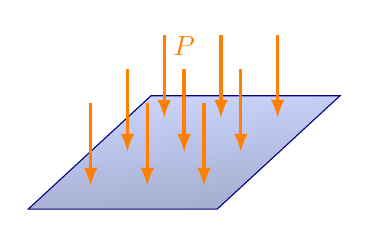
\begin{tikzpicture}[x={(1cm,0)},y={(0.65cm,0.6cm)},z={(0,1cm)},scale=1.5]
  \def\L{1.6} % cube side
  \def\P{0.7} % pressure size
  \draw[draw=blue!50!black,top color=blue!80!cyan!20!white,bottom color=blue!80!cyan!20!white!80!black,shading angle=5] (0,0,0) -- (\L,0,0) -- (\L,\L,0) -- ( 0,\L,0) -- cycle;
  \draw[-latex,orange,very thick] (0.5*\L,0.5*\L,1.01*\P) node[above=0.8] {$P$} --++ (0,0,-\P);
  \foreach \x/\y in {0.5/0.5,0.5/0.2,0.2/0.5,0.5/0.8,0.8/0.5,0.8/0.8,0.2/0.8,0.2/0.2,0.8/0.2}{
    \draw[-latex,orange,very thick] (\x*\L,\y*\L,1.01*\P) --++ (0,0,-\P);
  }
\end{tikzpicture}
\caption{圧力の模式}
\end{wrapfigure}

圧力（pressure）は単位面積あたりに加わる力の量のことで，記号$p$を用いる．
水圧は，基本的には\textbf{物体上にのしかかる水の重さ}である．
ここで重要なのは，水の密度$\rho$（単位体積あたりの質量）に依存するという点だ．

\begin{equation}
  p(z) = \rho zg
\end{equation}

で求められる．この数式を見れば分かるが底面積は\textbf{関係ない}．密度$\rho$のパラメータとしては，高さ$z$と重力加速度$g$のみに依存する．

\subsection{浮力}

\begin{wrapfigure}[15]{l}{0.36\textwidth}
\centering
\begin{tikzpicture}[scale=1.5]
  \def\Rx{1.1}      % tank horizontal radius
  \def\Ry{0.5}      % tank vertical radius
  \def\rx{0.22*\Rx} % column horizontal radius
  \def\ry{0.22*\Ry} % column vertical radius
  \def\H{2.6}       % height tank
  \def\h{0.94*\H}   % height draw=blue!50!black,top color=blue!80!cyan!10!white!90,bottom color=blue!80!cyan!10!white!90!black,shading angle=5
  \def\y{0.40*\H}   % vertical position piece
  \def\dy{0.10*\H}  % height piece
  
  % draw=blue!50!black,top color=blue!80!cyan!10!white!90,bottom color=blue!80!cyan!10!white!90!black,shading angle=5
  \draw[draw=blue!50!black,top color=blue!80!cyan!10!white!90,bottom color=blue!80!cyan!10!white!90!black,shading angle=5,top color=blue!80!cyan!10!white!90!black!90,bottom color=blue!80!cyan!10!white!90!black!90,middle color=blue!80!cyan!10!white!80,shading angle=90]
    (-\Rx,\h) -- (-\Rx,0) arc (180:360:{\Rx} and {\Ry}) -- (\Rx,\h);
  \draw[draw=blue!50!black,top color=blue!80!cyan!10!white!90,bottom color=blue!80!cyan!10!white!90!black,shading angle=5]
    (0,\h) ellipse ({\Rx} and {\Ry});
  
  % COLUMN + PIECE
  \draw[draw=blue!50!black,top color=blue!80!cyan!20!white,bottom color=blue!80!cyan!20!white!80!black,shading angle=5]
    (-\rx,\y) -- (-\rx,\y-\dy) arc (180:360:{\rx} and {\ry}) -- (\rx,\y);
  \draw[draw=blue!50!black,top color=blue!80!cyan!20!white,bottom color=blue!80!cyan!20!white!80!black,shading angle=5]
    (0,\y) ellipse ({\rx} and {\ry});
  \draw[draw=blue!50!black,top color=blue!80!cyan!20!white,bottom color=blue!80!cyan!20!white!80!black,shading angle=5,opacity=0.50,draw=none] % column
    (-\rx,\h) -- (-\rx,\y) arc (180:360:{\rx} and {\ry}) -- (\rx,\h) arc(360:180:{\rx} and {\ry}) -- cycle;
  \draw[blue!20!black,dashed,very thin,opacity=0.50] (-\rx,\y) -- (-\rx,\h) (\rx,\y) -- (\rx,\h);
  \draw[draw=blue!50!black,top color=blue!80!cyan!20!white,bottom color=blue!80!cyan!20!white!80!black,shading angle=5,opacity=0.50] % top column
    (0,\h) ellipse ({\rx} and {\ry});
  \draw[blue!30!black]
    (0,\h) ellipse ({\Rx} and {\Ry});
  
  % CONTAINER
  \draw[thick]
    (-\Rx,\H) -- (-\Rx,0) arc (180:360:{\Rx} and {\Ry}) -- (\Rx,\H);
  \draw[thick]
    (0,\H) ellipse ({\Rx} and {\Ry});
  
  % LABELS
  \node at ({-0.40*(\Rx+\rx)},{\y-0.5*\dy}) {$\tilde{V}$};
  \draw[Stealth-,thick] (0,\y-\ry) -- (0,1.5) node[above] {$\rho z_1 g$};
  \draw[Stealth-,thick] (0,\Ry+0.7*\dy) -- (0,0.1) node[below] {$\rho z_2 g$};
  \draw[latex-latex,thick] (1.2*\Rx,\y) --++ (0,\h-\y) node[midway,fill=white,inner sep=1] {$h$};
  
\end{tikzpicture}
\caption{水中で物体にかかる力}
\end{wrapfigure}

浮力が生じるのは，\textbf{水圧差}があるからである．図11でも示したが，物体を上から押す圧力と下から押す圧力は異なり，水圧の数式から下から押す圧力の方が大きい．次で数式で議論する．

\begin{equation}
  \bm{F} = \rho (z_2 - z_1)g
\end{equation}

底面積$S$には依存しないが，式変形のために導入し計算すると，

\begin{equation}
  \bm{F} = \rho \tilde{V}g
\end{equation}

ここでの$\tilde{V}$は水中での体積（volume）である．

\clearpage

\subsection{第12回\ 問題演習}

\begin{enumerate}
  \item 一辺の長さが10\ [cm]の立方体形の材木がある．材木の密度は0.75\ [g/cm]である．この材木を水に浮かべたとき，水面より上に出ている部分の高さを答えよ．
  \vs{5}
  \item[HINT] 材木に対する力のつりあいの式を用いよ．
  \item[] 水の密度は1.0\ [g/cm]である．

  \vs{10}

  水平右向きを$x$，鉛直上向きを$y$方向とし，重力ベクトルを成分表示すると，

  \begin{equation}
    \bm{F}_{\mathrm{gravity}} = (0 \quad - F_{\mathrm{gravity}})
  \end{equation}

  浮力ベクトルを成分表示すると，

  \begin{equation}
    \bm{F}_{\mathrm{buoyancy}} = (0 \quad F_{\mathrm{buoyancy}})
  \end{equation}

  材木は止まっていることより，力は釣り合っている．そのため，$F_{\mathrm{gravity}} = F_{\mathrm{buoyancy}}$である．
  また，物体の体積は一辺の長さが10\ [cm]の立方体形のため，$10^3\ [\mathrm{cm^3}]$である．
  求める高さを$h$とすると，アルキメデスの原理より$\tilde{V} = 10^2 \times (10-h)$である．

  \begin{equation}
  \renewcommand{\arraystretch}{2}
    \begin{array}{rl}
      & \rho V_{\mathrm{wood}}g = \rho \tilde{V}_{\mathrm{water}}g \\
      \Leftrightarrow & 0.75 \times 10^3 = 1.0 \times 10^2 \times (10-h) \\
      \Leftrightarrow & 0.75 = 10-h \\
      \Leftrightarrow & h = 2.5
    \end{array}
  \end{equation}

  \therefore\ 水面より上に出ている部分の高さは2.5\ [cm]．

  \vs{10}
  
  \item 水深3800\ [m]での水圧を[$\mathrm{Pa=N/m^2}$]で答えよ．真水として良い．
  \vs{5}
  \item[HINT] 水の密度は1\ [g/cm] = 何\ [kg/m]．

  \vs{10}

  この問いはそのまま公式に代入すればよい．

    \begin{equation}
  \renewcommand{\arraystretch}{2}
    \begin{array}{rcl}
      p(3800) &=& 9.8 \times 1.0 \times 10^3 \times 3800 \\
      &\simeq& 3.7 \times 10^7
    \end{array}
  \end{equation}

    \therefore\ 水深3800\ [m]での水圧は$3.7 \times 10^7$\ [Pa]．
    \footnote{解説はここまでにします．定期試験，頑張ってください．次項から，過去問の解説です．}
\end{enumerate}

\clearpage

\pagestyle{fancy}
\lhead{\ 試験解答}
\rhead{}
\cfoot{\thepage}

\section[定期試験]{定期試験\footnote{試験は過去問と{\color{cyan}ほぼ同じ問題が出題}されます．余計な勉強はせず，{\color{cyan}過去問を完璧}にしてください．}}

\begin{enumerate}[label={\LARGE \Roman*}]
    \item 水平な地面に立つ高さ$h=125$\ [m]のビルの屋上から，
    質量$m$のボールを，速さ$\bm{v}_0=3.0$\ [m/s]で水平かつ真東に打ち出した．
    このボールの運動を予測したい．下図のように地面に原点をとった2次元デカルト座標系を設定し，
    打ち出してからの時間を$t$\ [s]として，ボールの位置ベクトルをこの座標系で
    $\bm{r}(t)=(x(t) \quad y(t))$\ [m]と書くことにする．次の問に答えなさい．
    ただし，ボールに対する空気の影響は無視できる．
    問(1)と問(2)の答えには，なるべく数値を使わずに文字を使いなさい．
    問(3)と問(4)の数値の答えには，重力加速度の大きさ$\bm{g}=10\ [\mathrm{m/s^2}]$を使いなさい．

    \vs{10}

    \begin{center}
    \begin{tikzpicture}
        \fill[lightgray] (0,0) rectangle (-1,3);
        \draw[-latex,very thick] (-2,0)--(3,0) node[above]{$x$}node[right]{東}; %x軸
        \draw[-latex,very thick] (0,-0.5)--(0,4) node[right]{$y$}; %y軸
        \draw (0,0)node[below left]{O}; %原点
        \draw[semithick] (0,0) rectangle (-1,3)node[left]{$h=125$\ [m]};
        \draw (1.5,0)node[below]{地面};
        \fill (0,3) circle (0.08);
        \draw[-Stealth,semithick] (0,3)--(0.8,3)node[above right]{$\bm{v}_0=3.0$\ [m/s]};
        \draw (1,2.7) circle (0.08);
        \draw (1.5,2.4) circle (0.08)node[right]{$(x(t),y(t))$};
        \draw (2,1.7) circle (0.08);
    \end{tikzpicture}
    \end{center}

    \vs{10}
    
    \begin{enumerate}[label=(\arabic*)]
        \item 問題文で用意された座標系と函数を使って，打ち出されてから地面に着くまでの間のボールの\textbf{運動方程式}と
        ボールの\textbf{初期条件}を書きなさい．

        \vspace{5pt}        

        地面に着くまでにボールにはたらく力は重力のみである．従って，地面に着くまでの間のボールの運動方程式は次である．

        \begin{equation}
            m(\ddot{x}(t) \quad \ddot{y}(t))=(0 \quad -mg) \quad \Leftrightarrow \quad
            \begin{cases}
                m \ddot{x}(t)=0 \\
                m \ddot{y}(t)=-mg
            \end{cases}
        \end{equation}

        時刻$t=0$には，ボールは位置$(0,h)$におり，かつ，速度が$(v_0,0)$だったので，初期条件は次である．

        \begin{equation}
            x(0)=0,\ y(0)=h  \quad \Leftrightarrow \quad
            \dot{x}(0)=v_0,\ \dot{y}(0)=0
        \end{equation}

        \clearpage

        \item 問1の方程式と条件を解いて，空中に飛んでいるボールの\textbf{運動}，つまり，函数$x(t)$と$y(t)$を答えなさい．
        
        \vspace{5pt}

        (1)の運動方程式より，$A$～$D$を任意の定数として，函数$x(t)$と$y(t)$が次のように，一旦，無数に求まる．

        \begin{equation}
            \begin{cases}
                m \ddot{x}(t)=0 \\
                m \ddot{y}(t)=-g
            \end{cases}
            \quad \Leftrightarrow \quad
            \begin{cases}
                x(t)=At+B \\
                y(t)=-\dfrac{1}{2}gt^2+Ct+D
            \end{cases}
        \end{equation}

        ここで，(1)の初期条件より$A$～$D$は決定され，$A=v_0$，$B=0$，$C=0$，$D=h$である．
        問題のボールの運動に対応する函数は次である．

        \begin{equation}
            \begin{cases}
                x(t)=v_0t \\
                y(t)= \dfrac{1}{2}gt^2+h
            \end{cases}
        \end{equation}

        \vspace{5pt}

        \item 打ち出してから$2.0$\ [s]後のボールの\textbf{位置}と\textbf{速度}を答えなさい．

        \vspace{5pt}

        (2)で得た式に$t=2.0$\ [s]を代入する．

        \begin{equation}
            \begin{cases}
                x(2)=3.0 \times 2.0=6.0\ [\mathrm{m}] \\
                y(2)=-\dfrac{1}{2} \cdot 10 \times 2.0^2+125=105\ [\mathrm{m}]
            \end{cases}
        \end{equation}

        位置は与えられた座標系で\ $(6.0 \quad 105)$\ [m]

        \vspace{5pt}

        (2)の式を1回微分した式に$t=2.0$\ [s]を代入する．

        \begin{equation}
            \begin{cases}
                \dot{x}(t)=v_0 \\
                \dot{y}(t)=-gt
            \end{cases}
            \quad \Rightarrow \quad
            \begin{cases}
                \dot{x}(2)=3.0\ [\mathrm{m/s}] \\
                \dot{y}(2)=-10 \times 2.0 = -20\ [\mathrm{m/s}]
            \end{cases}
        \end{equation}

        速度は与えられた座標系の成分表示で $(3.0 \quad -20)$\ [m/s]

        \clearpage

        \item 問題のボールが地面に衝突する\textbf{時刻}と\textbf{位置}を答えなさい．
        
        \vspace{5pt}

        地面は$y=0$であるから，衝突する時刻は$y(T)=0$となる$T$を正の範囲で求めたらよい．

        \vspace{-15pt}

        \begin{equation}
          \renewcommand{\arraystretch}{3}
            \begin{array}{ccc}
                & y(T)=0 \quad \Leftrightarrow \quad -\dfrac{1}{2}gT^2+h=0 \\
                \Leftrightarrow \quad & T=\sqrt{\dfrac{2h}{g}} = \sqrt{\dfrac{2 \times 125\ [\mathrm{m}]}{10\ [\mathrm{m/s^2}]}}=5.0\ [\mathrm{m}]
            \end{array}
        \end{equation}

        衝突する地点は，時刻$T$でのボールの位置，すなわち，与えられた座標系で$(x(T),0)$である．
        \begin{equation}
            x(T)=v_0T=3.0\ [\mathrm{m/s}] \times 5.0\ [\mathrm{s}]=15\ [\mathrm{m}]
        \end{equation}
        より，ビルの根本から真東に15\ [m]の地点である．
        \vspace{5pt}
    \end{enumerate}

\clearpage

    \item 水平から角度$23^\circ$の\textbf{なめらかな}斜面に，質量$m=5.0$\ [kg]の小物体が糸が引かれて静止している．
    糸と斜面は平行である．糸が小物体を引く力$\bm{T}$の大きさ$T$と小物体にはたらく垂直抗力$\bm{N}$の大きさ$N$を，
    適切な単位で答えなさい．\textbf{途中の説明には図の書き込みを併用してよい}．必要があれば，$\sin 23^\circ = 0.39$，$\cos 23^\circ = 0.92$を使ってよい．
    重力加速度の大きさは$\bm{g}=10\ [\mathrm{m/s^2}]$とする．

    \vs{20}

    \begin{center}
      \begin{tikzpicture}
        \coordinate (A) at (5,3.5) {};
        \coordinate (B) at (0,0) {};
        \coordinate (C) at (5,0) {};
        \draw[thick] (A)--(B)--(C);
        \pic[draw,"$23^{\circ}$",angle radius=8mm,angle eccentricity=1.7] {angle = C--B--A};
        \draw[semithick,fill=lightgray,rotate=35] (1.8,0) rectangle(3,1);
        \draw[semithick,fill=black,rotate=35] (5,0) rectangle(5.1,1);
        \draw[rotate=35] (3,0.5)--(5,0.5)node[above] at ($(3,0.5)!0.5!(5,0.5)$){糸};
      \end{tikzpicture}
    \end{center}

    \vs{20}

    図のように，水平面の適当な所に原点をとり，斜面に平行上向きを$x$方向，斜面に垂直上向きを$y$方向とする．
    この座標系は慣性座標系である．小物体にはたらく力は重力$\bm{G}$と，糸が引く力$\bm{T}$と，垂直抗力$\bm{N}$である．
    図のように，重力$\bm{G}$は鉛直下向き，糸が引く力$\bm{T}$は斜面平行上向き，垂直抗力$\bm{N}$は斜面垂直上向きである．
    物体は慣性座標系に対して静止しているのだから，「力のついあい」$\bm{G}+\bm{T}+\bm{N}=\bm{0}$が成り立っている．
    設定した座標系で物体にはたらく3つの力を成分表示すると次のようになる．

    \begin{equation}
        \bm{G}=(-mg\sin23^{\circ} \quad -mg\cos23^{\circ})
        \qquad
        \bm{T}=(T \quad 0)
        \qquad
        \bm{N}=(0 \quad N)
    \end{equation}

    これらの成分表示を使って「力のついあい」を表すと次のようになる．

    \begin{equation}
        \bm{G}+\bm{T}+\bm{N}=(T-mg\sin23^{\circ} \quad N-mg\cos23^{\circ})=(0 \quad 0)
    \end{equation}

    これらの方程式を解いて，求める力の強さ$T$と$N$が次のように得られる．

    \begin{equation}
      \renewcommand{\arraystretch}{2}
        \begin{array}{rcccccl}
            T &=& mg\sin23^{\circ} &=& 5.0\ [\mathrm{kg}] \times 10\ [\mathrm{m/s^2}] \times 0.39 &=& 19.5\ [\mathrm{N}] \\
            N &=& mg\cos23^{\circ} &=& 5.0\ [\mathrm{kg}] \times 10\ [\mathrm{m/s^2}] \times 0.92 &=& 46.0\ [\mathrm{N}]
        \end{array}
    \end{equation}

\clearpage

    \item 質量不明の小物体を地面から$\bm{v}_0=15$\ [m/s]である角度に打ち出すと，最高点の地面からの高さは$H=10$\ [m]であった．
    物質の最高点での\textbf{速さ}$\bm{v}$を答えなさい．重力加速度の大きさは$\bm{g}=10\ [\mathrm{m/s^2}]$とする．空気の影響は無視できる．

    \vspace{5pt}

    ボールの質量を$m$と表し，重力による位置エネルギー$U$を基準に地面にとる．
    投げた瞬間と最高点の瞬間のボールの運動エネルギー$K$と位置エネルギー$U$は次である．

    \begin{equation}
      \renewcommand{\arraystretch}{2}
      \begin{array}{ccccl}
        \hline
        \multirow{2}{*}{投げた瞬間} & 運動エネルギー & K_1 &=& \dfrac{1}{2}m\bm{v}_0^2 \\
                  & 位置エネルギー & U_1 &=& \bm{0} \\
        \hline
        \multirow{2}{*}{最高点の瞬間} & 運動エネルギー & K_2 &=& \dfrac{1}{2}m\bm{v}^2 \\
                    & 位置エネルギー & U_2 &=& m\bm{g}H \\
        \hline
      \end{array}
    \end{equation}


    ボールには重力の他に力がはたらいていないから，力学的エネルギー$E$は保存する．

    \begin{equation}
      \renewcommand{\arraystretch}{1.5}
        \begin{array}{rrcl}
            & E_1 &=& E_2 \\
            \Leftrightarrow & \dfrac{1}{2}m\bm{v}_0^2 &=& \dfrac{1}{2}m\bm{v}^2 + m\bm{g}H \\
            \Leftrightarrow & \bm{v}_0^2              &=& \bm{v}^2 + 2\bm{g}H \\
            \Leftrightarrow & \bm{v}^2                &=& \bm{v}_0 - 2\bm{g}H \\
                          = & 225 - 200               &=& 25\ [\mathrm{m^2/s^2}] \\
            \Leftrightarrow & \bm{v}                  &=& 5.0\ [\mathrm{m/s}]
        \end{array}
    \end{equation}

    \vspace{5pt}

    \item 次の文章のカッコに適当な単語を埋めなさい．
    
    \vspace{5pt}

    \begin{enumerate}[label=(\arabic*)]
        \item 電車に乗っていると，減速中に上半身を進行方向に押し付けられるように感じる．
        この力は（\ \textbf{\color{cyan}慣性力}\ ）と呼ばれるが，本物の力ではない．
        実際，この現象を地面を基準に考えると，身体は等速度を続けようとする慣性の法則に，
        電車の床に着いている足だけが電車と共に減速するから，上半身が前のめりになるだけなのである．
        このような見かけの力であっても，（\ \textbf{\color{cyan}非慣性}\ ）座標系を採用して運動を調べる場合に役に立つ．

        \item 物体の軸の回りの回転運動を考えるときは，力よりも（\ \textbf{\color{cyan}力のモーメント}\ ）と呼ばれるベクトルの方が便利である．
        \item このベクトルの大きさは，力の大きさの他に，軸から力の作用点までの（\ \textbf{\color{cyan}距離}\ ）にも比例する．
    \end{enumerate}

    \vspace{5pt}

    \item 授業や試験の感想，要望，文句，その他，何でもよいので書きなさい．

    \vspace{5pt}

    　先生に対しての苦情を書くと減点されます．先生を褒める言葉を記述して下さい．

\end{enumerate}

\clearpage

\pagestyle{fancy}
\lhead{}
\rhead{}
\cfoot{\thepage}
\renewcommand{\headrulewidth}{0.0pt}

\setcounter{page}{1}

\begin{enumerate}[label={\LARGE \Roman*}]
    \item 水平な地面に立つ高さ$h=125$\ [m]のビルの屋上から，
    質量$m$のボールを，速さ$\bm{v}_0=3.0$\ [m/s]で水平かつ真東に打ち出した．
    このボールの運動を予測したい．下図のように地面に原点をとった2次元デカルト座標系を設定し，
    打ち出してからの時間を$t$\ [s]として，ボールの位置ベクトルをこの座標系で
    $\bm{r}(t)=(x(t) \quad y(t))$\ [m]と書くことにする．次の問に答えなさい．
    ただし，ボールに対する空気の影響は無視できる．
    問(1)と問(2)の答えには，なるべく数値を使わずに文字を使いなさい．
    問(3)と問(4)の数値の答えには，重力加速度の大きさ$\bm{g}=10\ [\mathrm{m/s^2}]$を使いなさい．

    \vs{10}

    \begin{center}
    \begin{tikzpicture}
        \fill[lightgray] (0,0) rectangle (-1,3);
        \draw[-latex,very thick] (-2,0)--(3,0)node[above]{$x$}node[right]{東}; %x軸
        \draw[-latex,very thick] (0,-0.5)--(0,4)node[right]{$y$}; %y軸
        \draw (0,0)node[below left]{O}; %原点
        \draw[semithick] (0,0) rectangle (-1,3)node[left]{$h=125$\ [m]};
        \draw (1.5,0)node[below]{地面};
        \fill (0,3) circle (0.08);
        \draw[-Stealth,semithick] (0,3)--(0.8,3)node[above right]{$\bm{v}_0=3.0$\ [m/s]};
        \draw (1,2.7) circle (0.08);
        \draw (1.5,2.4) circle (0.08)node[right]{$(x(t),y(t))$};
        \draw (2,1.7) circle (0.08);
    \end{tikzpicture}
    \end{center}

    \vs{10}
    
    \begin{enumerate}[label=(\arabic*)]
        \item 問題文で用意された座標系と函数を使って，打ち出されてから地面に着くまでの間のボールの\textbf{運動方程式}と
        ボールの\textbf{初期条件}を書きなさい．

        \vspace{5pt}        

        地面に着くまでにボールにはたらく力は重力のみである．従って，地面に着くまでの間のボールの運動方程式は次である．

        \vs{120}

        時刻$t=0$には，ボールは位置$(0,h)$におり，かつ，速度が$(\bm{v}_0,0)$だったので，初期条件は次である．

\clearpage

        \item 問1の方程式と条件を解いて，空中に飛んでいるボールの\textbf{運動}，つまり，函数$x(t)$と$y(t)$を答えなさい．
        
        \vs{200}

        \item 打ち出してから$2.0$\ [s]後のボールの\textbf{位置}と\textbf{速度}を答えなさい．

        \vs{200}

        \item 問題のボールが地面に衝突する\textbf{時刻}と\textbf{位置}を答えなさい．
        
    \end{enumerate}

\clearpage

    \item 水平から角度$23^\circ$の\textbf{なめらかな}斜面に，質量$m=5.0$\ [kg]の小物体が糸が引かれて静止している．
    糸と斜面は平行である．糸が小物体を引く力$\bm{T}$の大きさ$T$と小物体にはたらく垂直抗力$\bm{N}$の大きさ$N$を，
    適切な単位で答えなさい．\textbf{途中の説明には図の書き込みを併用してよい}．必要があれば，$\sin 23^\circ = 0.39$，$\cos 23^\circ = 0.92$を使ってよい．
    重力加速度の大きさは$\bm{g}=10\ [\mathrm{m/s^2}]$とする．

    \vs{20}

    \begin{center}
      \begin{tikzpicture}
        \coordinate (A) at (5,3.5) {};
        \coordinate (B) at (0,0) {};
        \coordinate (C) at (5,0) {};
        \draw[thick] (A)--(B)--(C);
        \pic[draw,"$23^{\circ}$",angle radius=8mm,angle eccentricity=1.7] {angle = C--B--A};
        \draw[semithick,fill=lightgray,rotate=35] (1.8,0) rectangle(3,1);
        \draw[semithick,fill=black,rotate=35] (5,0) rectangle(5.1,1);
        \draw[rotate=35] (3,0.5)--(5,0.5)node[above] at ($(3,0.5)!0.5!(5,0.5)$){糸};
      \end{tikzpicture}
    \end{center}

    \vs{200}

    \item 質量不明の小物体を地面から$\bm{v}_0=15$\ [m/s]である角度に打ち出すと，最高点の地面からの高さは$H=10$\ [m]であった．
    物質の最高点での\textbf{速さ}$\bm{v}$を答えなさい．重力加速度の大きさは$\bm{g}=10\ [\mathrm{m/s^2}]$とする．空気の影響は無視できる．

\clearpage

    \item 次の文章のカッコに適当な単語を埋めなさい．
    
    \vs{20}

    \begin{enumerate}[label=(\arabic*)]
        \item 電車に乗っていると，減速中に上半身を進行方向に押し付けられるように感じる．
        この力は（\hs{50}）と呼ばれるが，本物の力ではない．
        実際，この現象を地面を基準に考えると，身体は等速度を続けようとする慣性の法則に，
        電車の床に着いている足だけが電車と共に減速するから，上半身が前のめりになるだけなのである．
        このような見かけの力であっても，（\hs{50}）座標系を採用して運動を調べる場合に役に立つ．

        \item 物体の軸の回りの回転運動を考えるときは，力よりも（\hs{80}）と呼ばれるベクトルの方が便利である．
        \item このベクトルの大きさは，力の大きさの他に，軸から力の作用点までの（\hs{50}）にも比例する．
    \end{enumerate}

    \vs{20}

    \item 授業や試験の感想，要望，文句，その他，何でもよいので書きなさい．

\end{enumerate}

\end{document}